\chapter{Appendix for Part II: Machine Learning Applications to Chemistry}
\renewcommand\thefigure{\thesection.\arabic{figure}}
\renewcommand\thetable{\thesection.\arabic{table}}


\section{Supplementary Information for Chpater 4: Variational Autoencoders for Optimization in Molecular Space}

This section contains peripheral findings including statistics on the latent space, reconstruction accuracy, training robustness with respect to dataset size, and more sampling interpolation examples.

\begin{table}[h]
\centering
\caption{Percentage of successfully decoding of latent representation after 1000 attempts for 1000 molecules from the traning set, 1000 validation molecules randomly chosen from ZINC and a 1000 validation molecules randomly chosen from eMolecules. Both VAEs perform very well for training data, and they are well transferable within molecules of the same class outside the training data, as evidence by the good validation performance of the ZINC VAE and the underperformance of the QM9 VAE against real-life small molecules.}
\begin{tabular}{lp{1cm}lp{1cm}lp{1cm}}
\hline
Dataset & ZINC & QM \\
\hline
Training set & 92.1 & 99.6 \\
Test set & 90.7 & 99.4 \\
ZINC & 91.0 & 1.4 \\
eMolecules & 83.8 & 8.8 \\
\hline
\end{tabular}
\label{tab:recovery statistics}
\end{table}[h]

\begin{table}[h]
\centering
\caption{Percentage of 5000 randomly-selected latent points that decode to valid molecules after 1000 attempts}
\begin{tabular}{lp{1cm}lp{1cm}lp{1cm}}
Dataset & ZINC & QM \\
\hline
Decoding probability & 73.9 & 79.3 \\
\end{tabular}
\label{tab:random_sampling_statistics}
\end{table}


\begin{table}[h]
\centering
\caption{ Variational autoencoder performance over different sizes of datasets. Training and tests were performed using randomly selected molecules from the ZINC dataset, the values reported here are the scores from the validation set. The categorical accuracy reflects the percentage of characters in the output SMILES that were accurately reconstructed. Mean Absolute Errors (MAE) are reported for QED and logP properties. Performance significantly decreases if only ~$10^5$ molecules are used for training.}
\begin{tabular}{cp{2cm}cp{2cm}cp{2cm}cp{2cm}}
\hline
Training set size &  Categorical Accuracy & logP MAE & QED MAE\\
\hline
225,000 & 99.3\% & 0.15 & 0.054 \\
175,000 & 99.0\% & 0.18 & 0.076 \\
125,000 & 98.5\% & 0.15 & 0.076 \\
25,000 & 91.6\% & 0.23 & 0.079 \\
\hline
\end{tabular}
\label{tab:Accuracy_by_training_size}
\end{table}

\begin{figure}[h]
\centering
  \begin{subfigure}{0.45\textwidth}
    \caption{}
    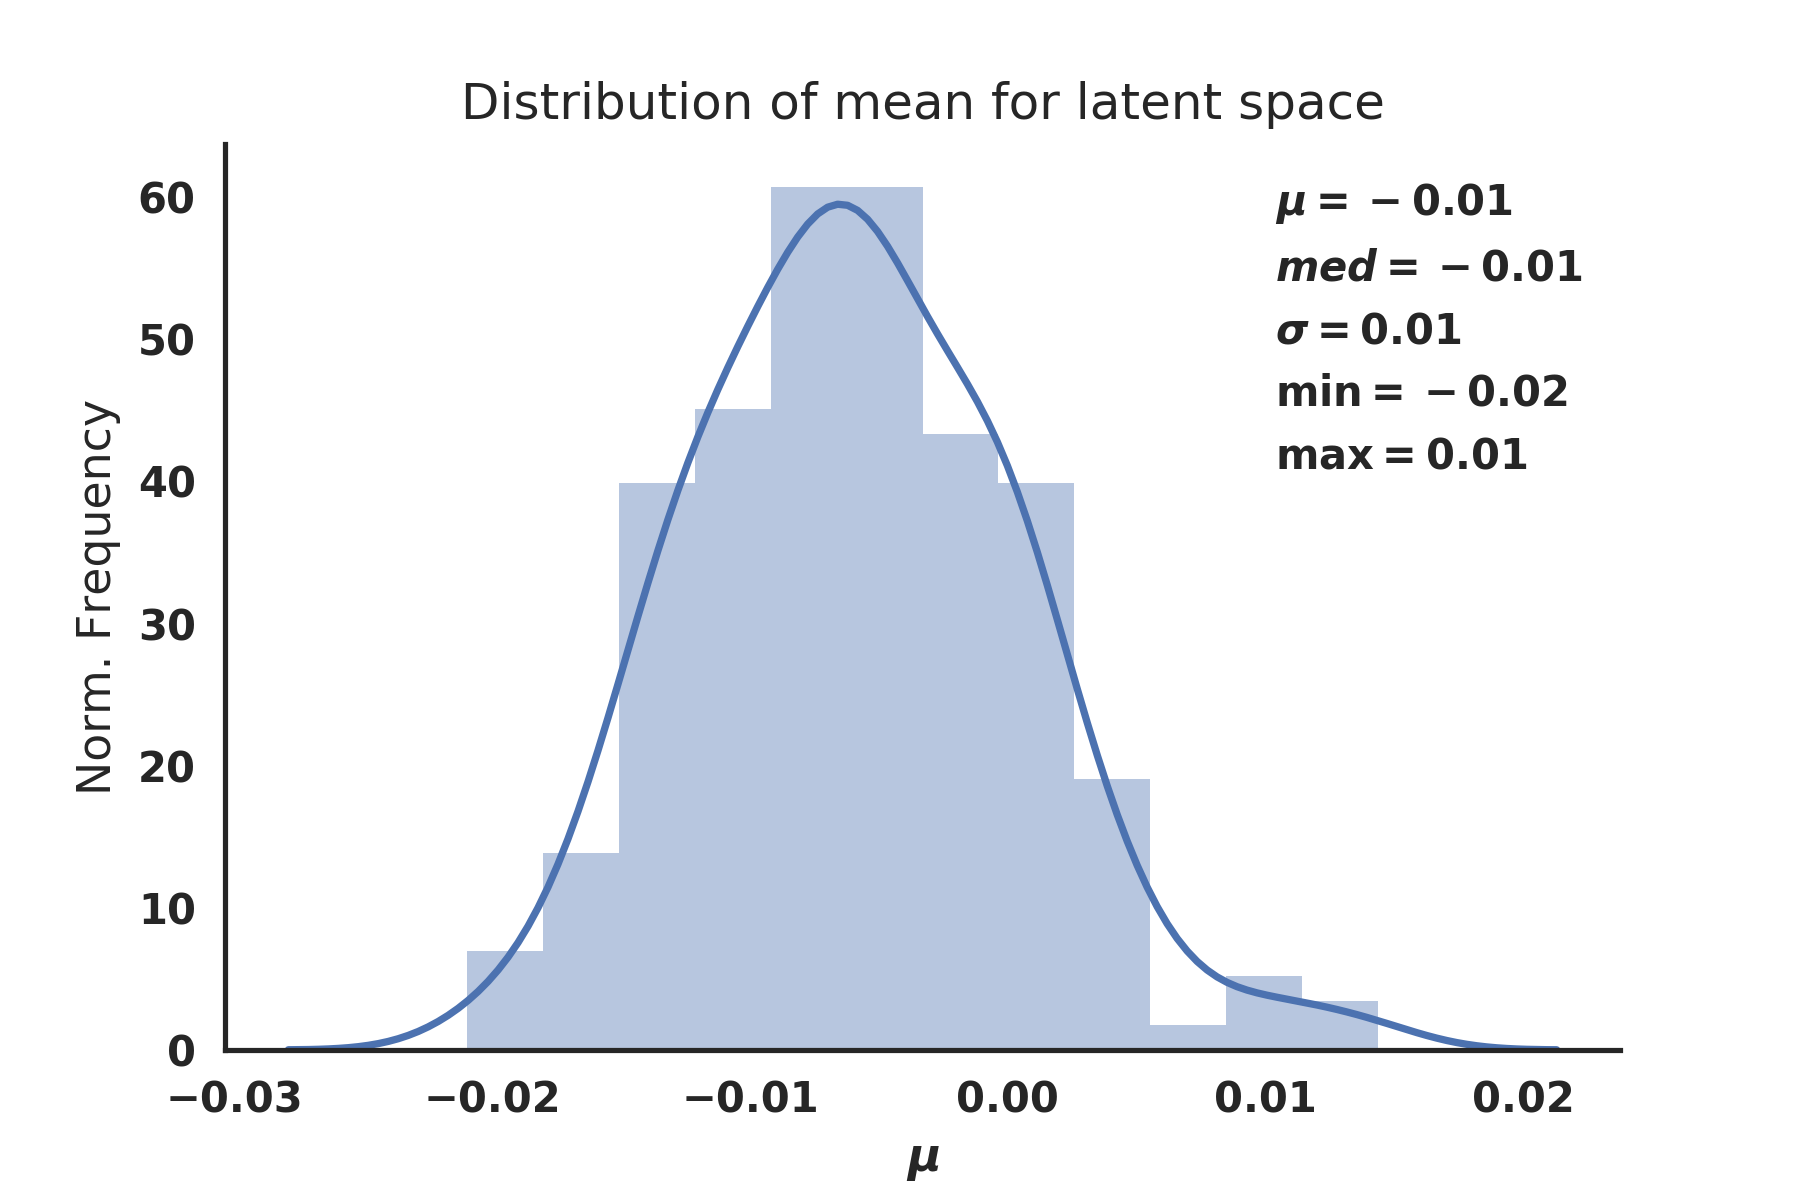
\includegraphics[width=\textwidth]{./mean_Z.png}
  \end{subfigure}
  \begin{subfigure}{0.45\textwidth}
    \caption{}
    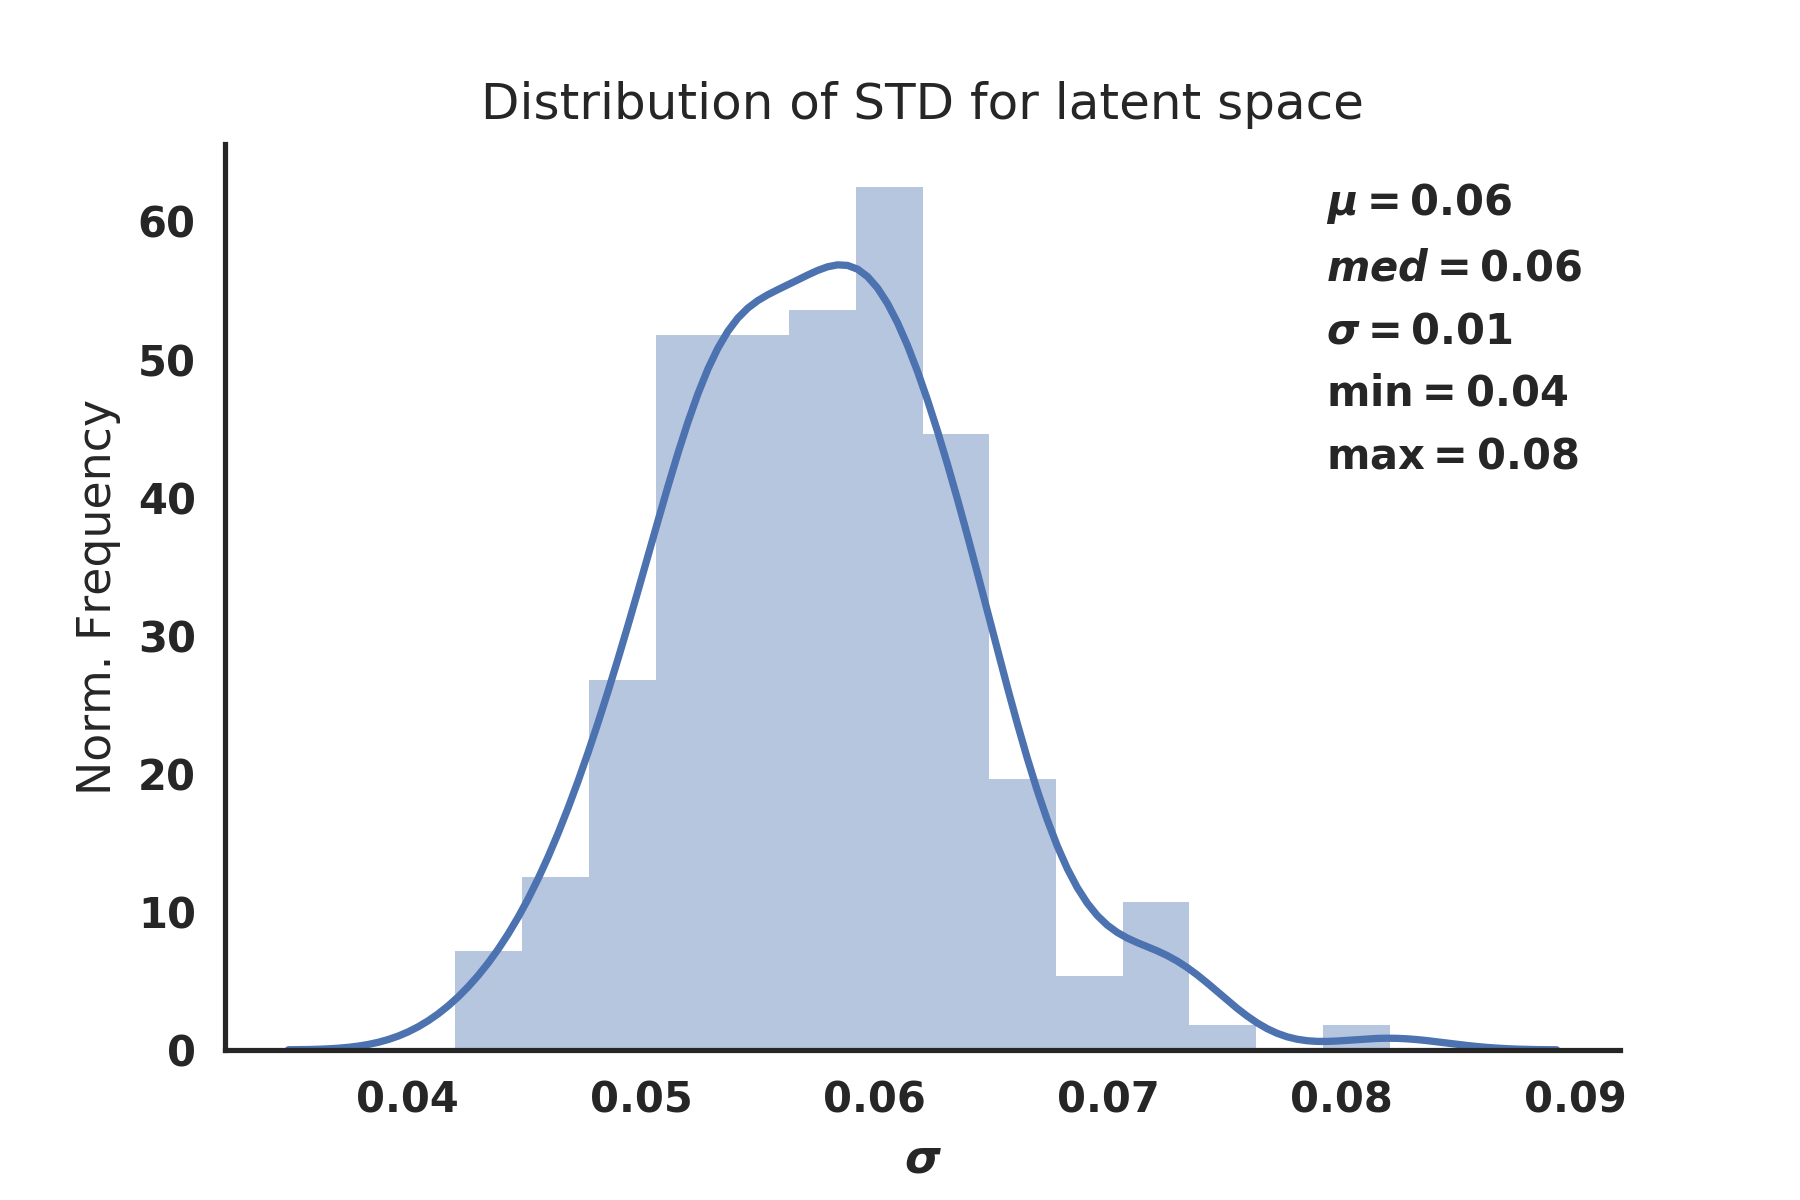
\includegraphics[width=\textwidth]{./STD_Z.png}
  \end{subfigure}
  \vspace{1em}
  \begin{subfigure}{0.45\textwidth}
    \caption{}
    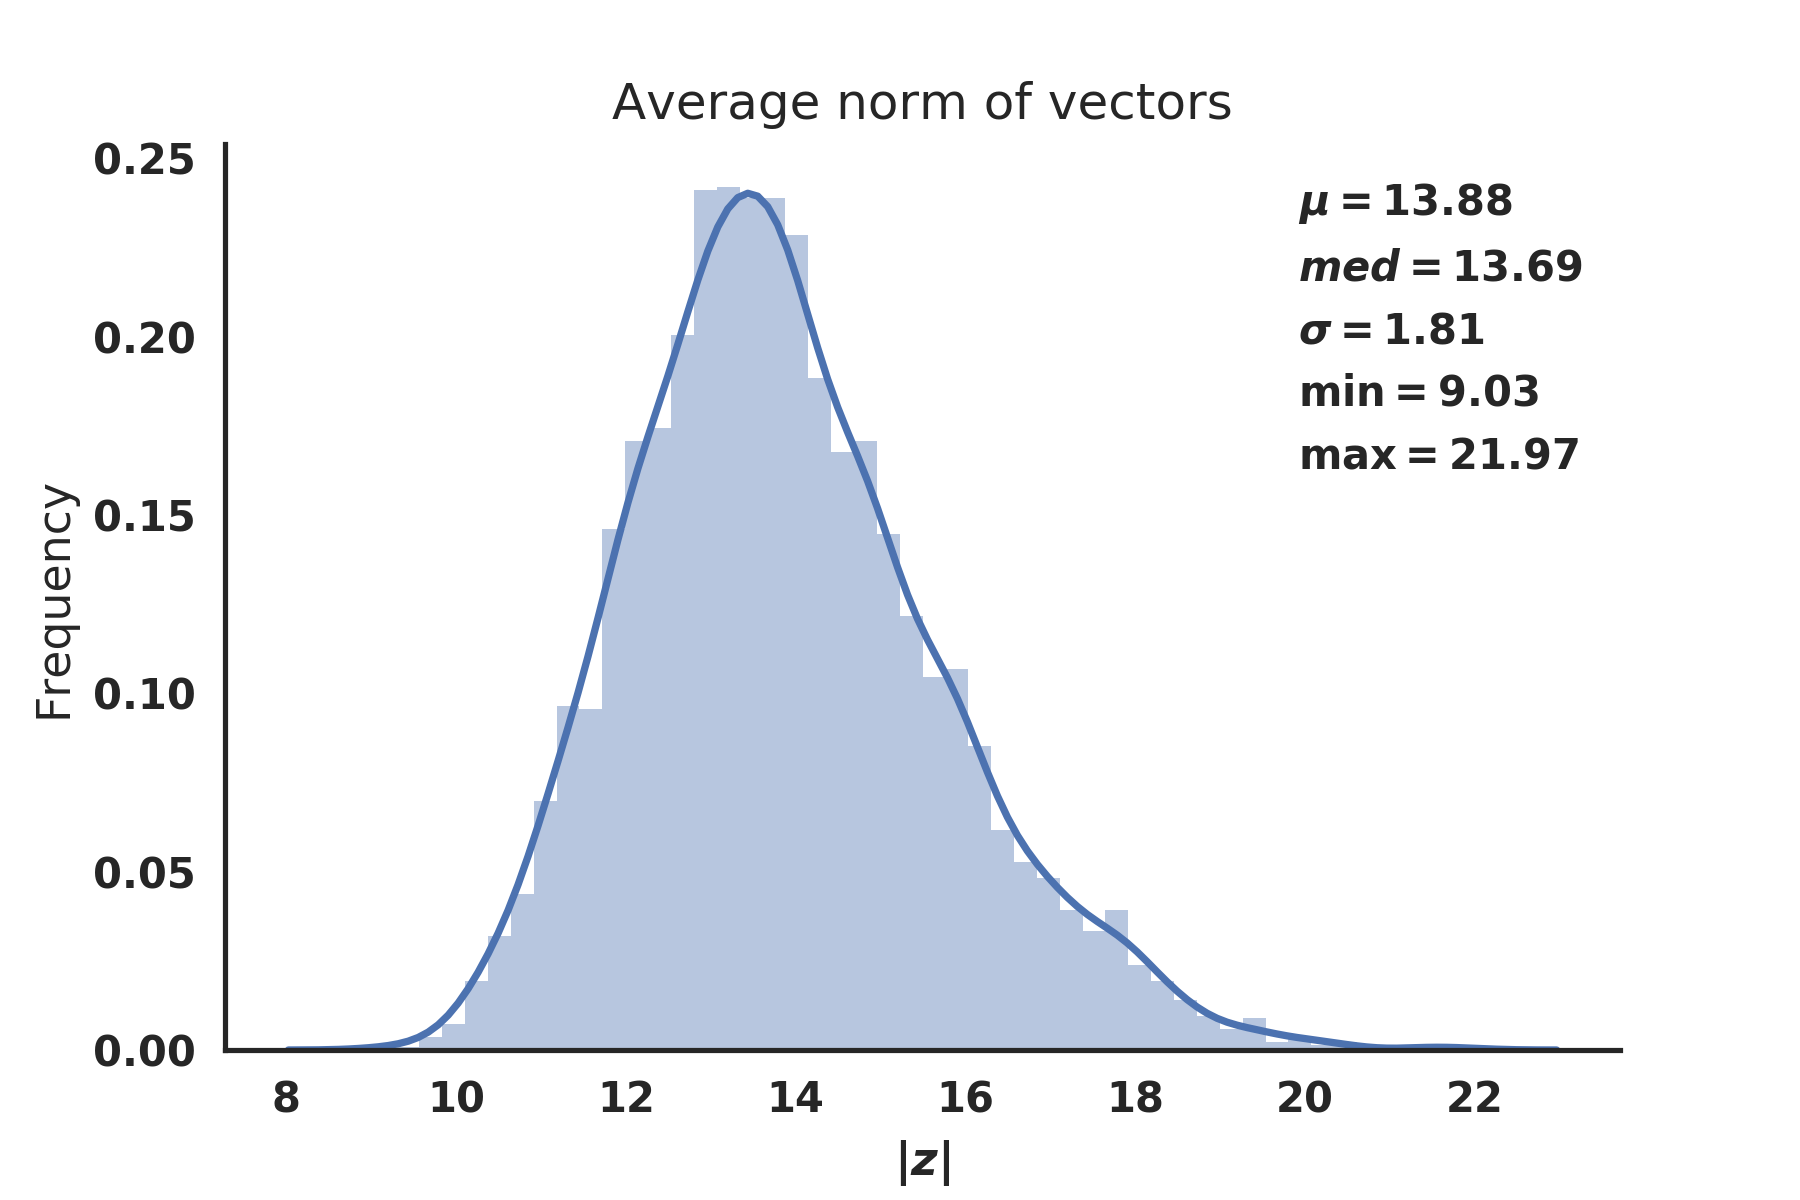
\includegraphics[width=\textwidth]{./norm_Z.png}
  \end{subfigure}
  \begin{subfigure}{0.45\textwidth}
    \caption{}
    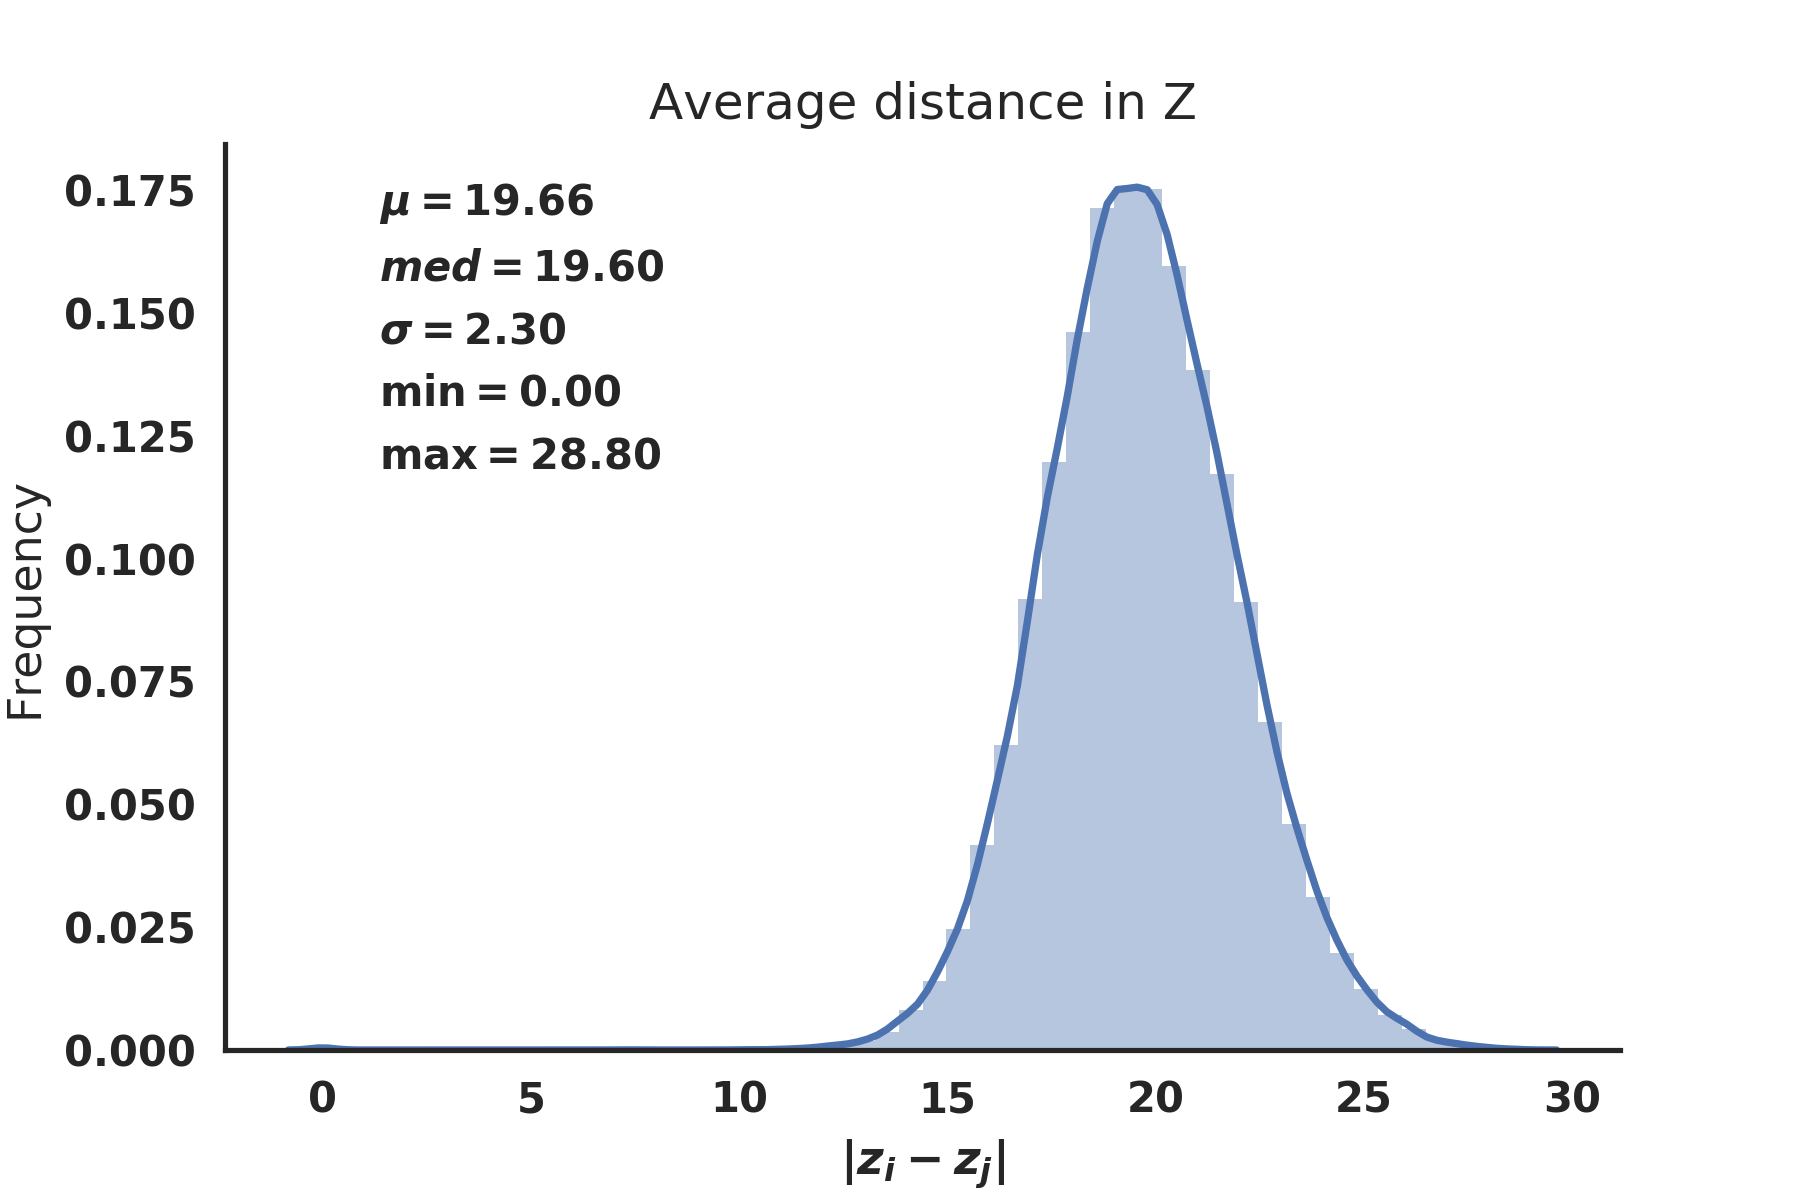
\includegraphics[width=\textwidth]{./distance_Z.png}
  \end{subfigure}
\caption[Latent Space Distribution Statistics]{Distribution and statistics of (a) the mean of latent space coordinates (b) standard deviation of latent space coordinates (c) norm of latent space coordinates of the encoded representation of randomly selected molecules from the ZINC validation set. (d) Distribution of Euclidean distances between random pairs of validation molecules in the ZINC VAE }
\label{fig:ls_stats}
\end{figure}


\begin{figure}
\centering
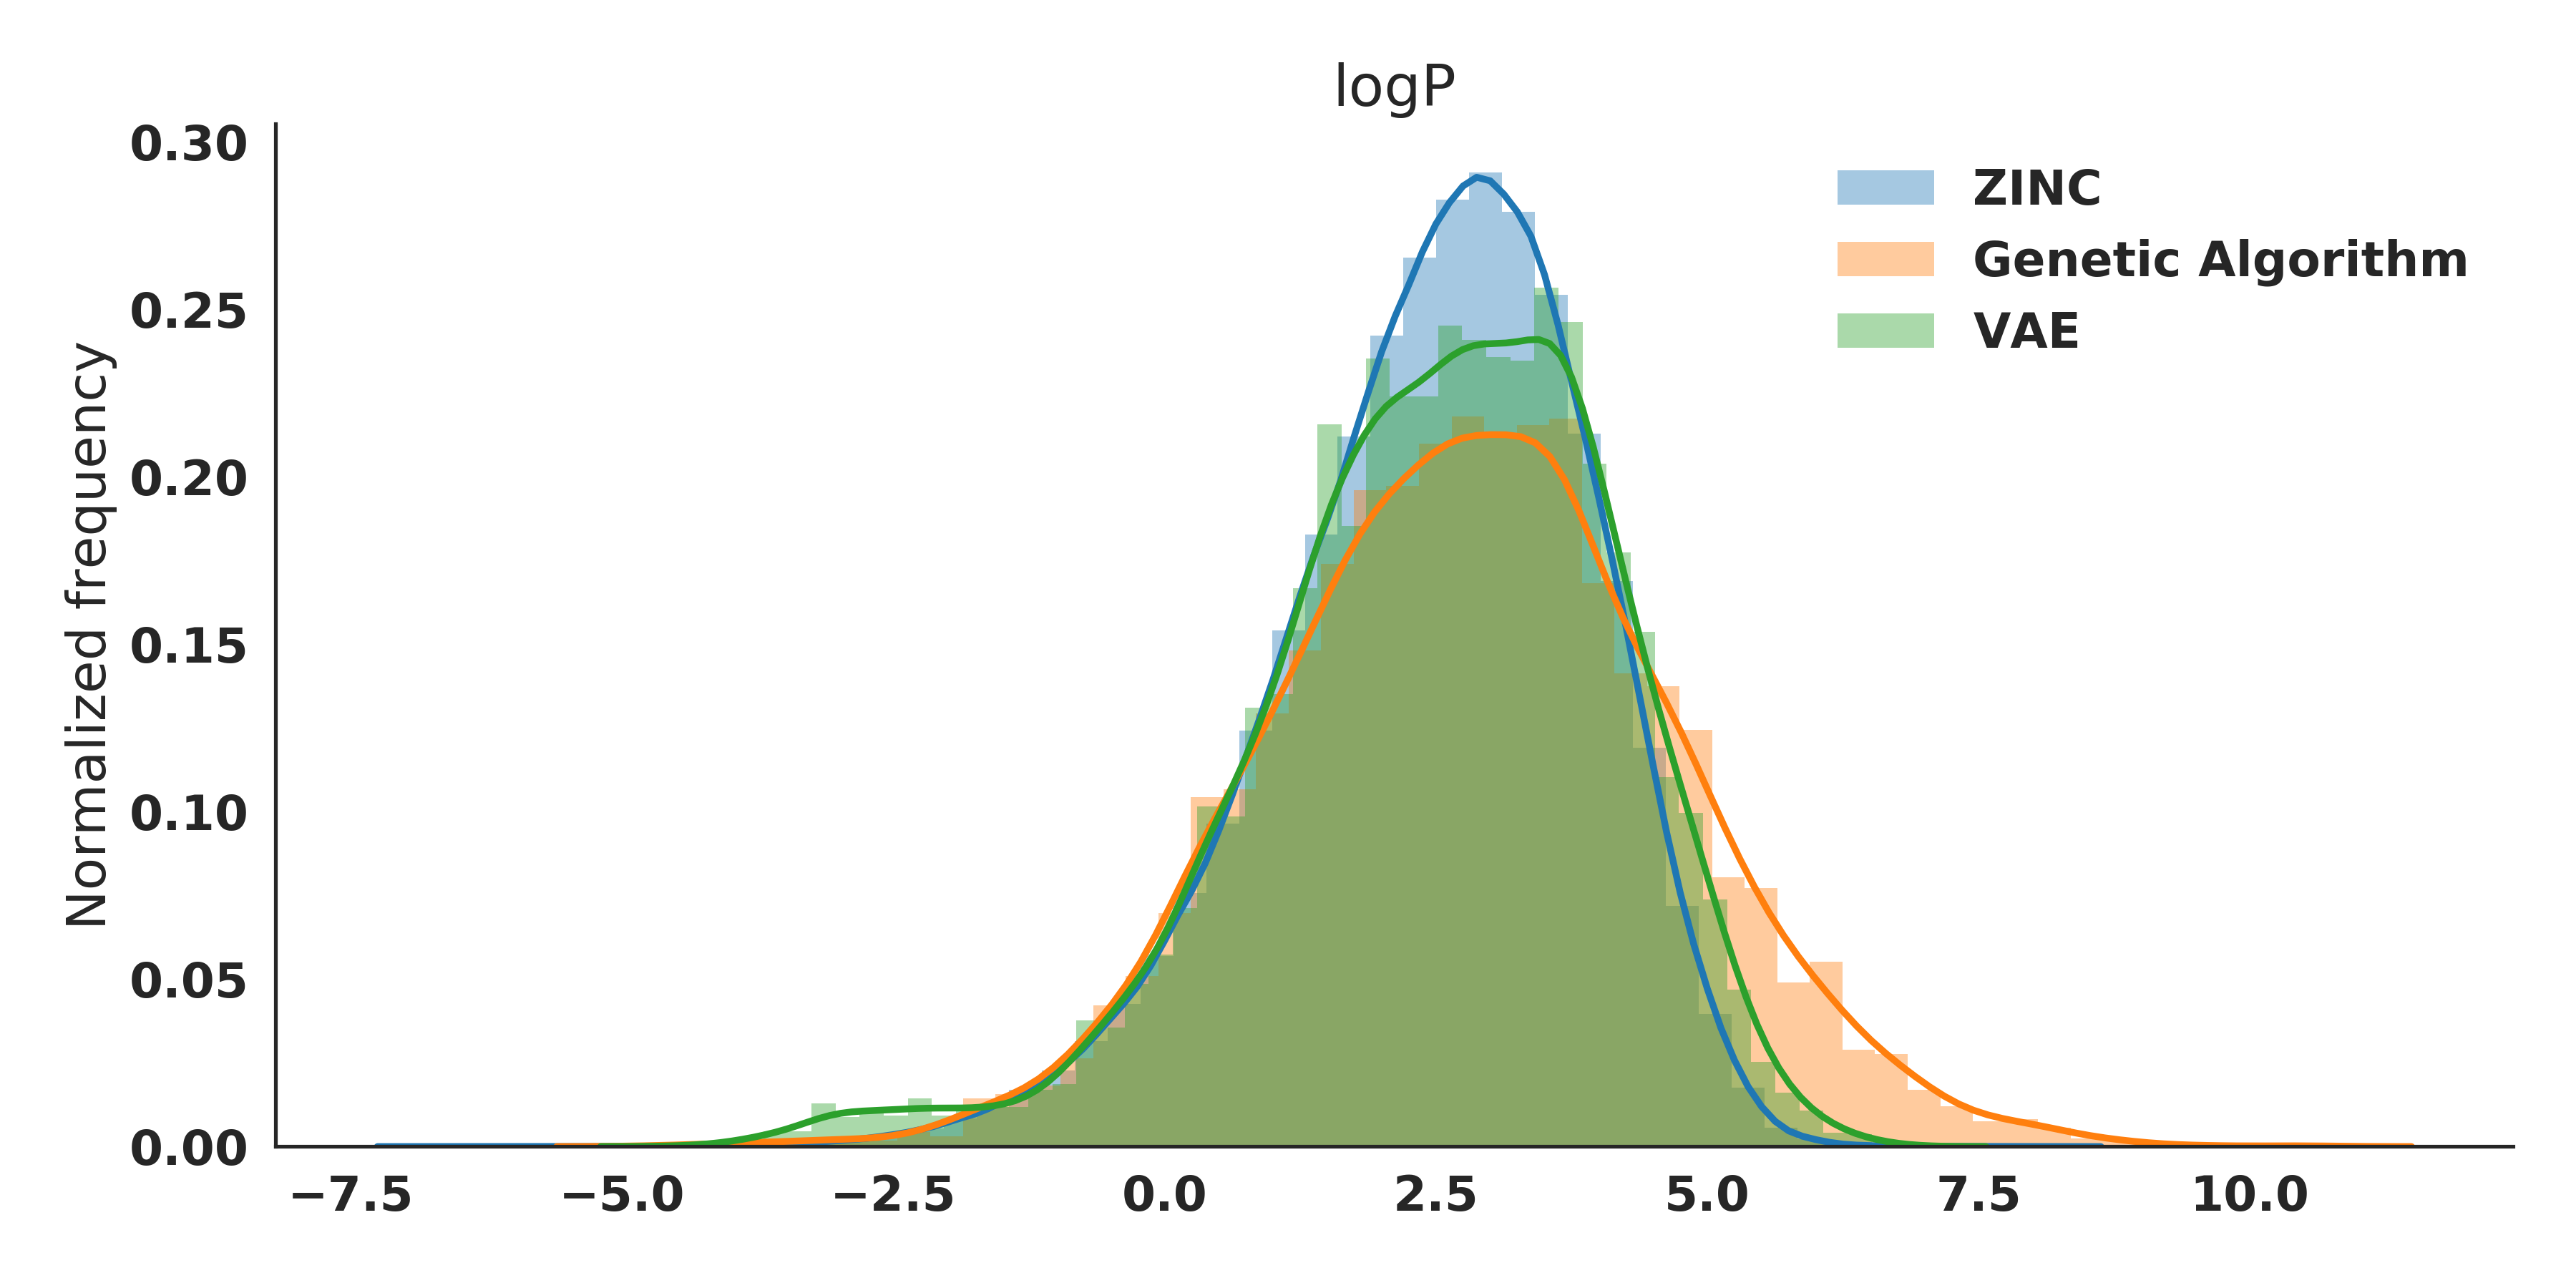
\includegraphics[width=0.3\columnwidth]{./logP.png}
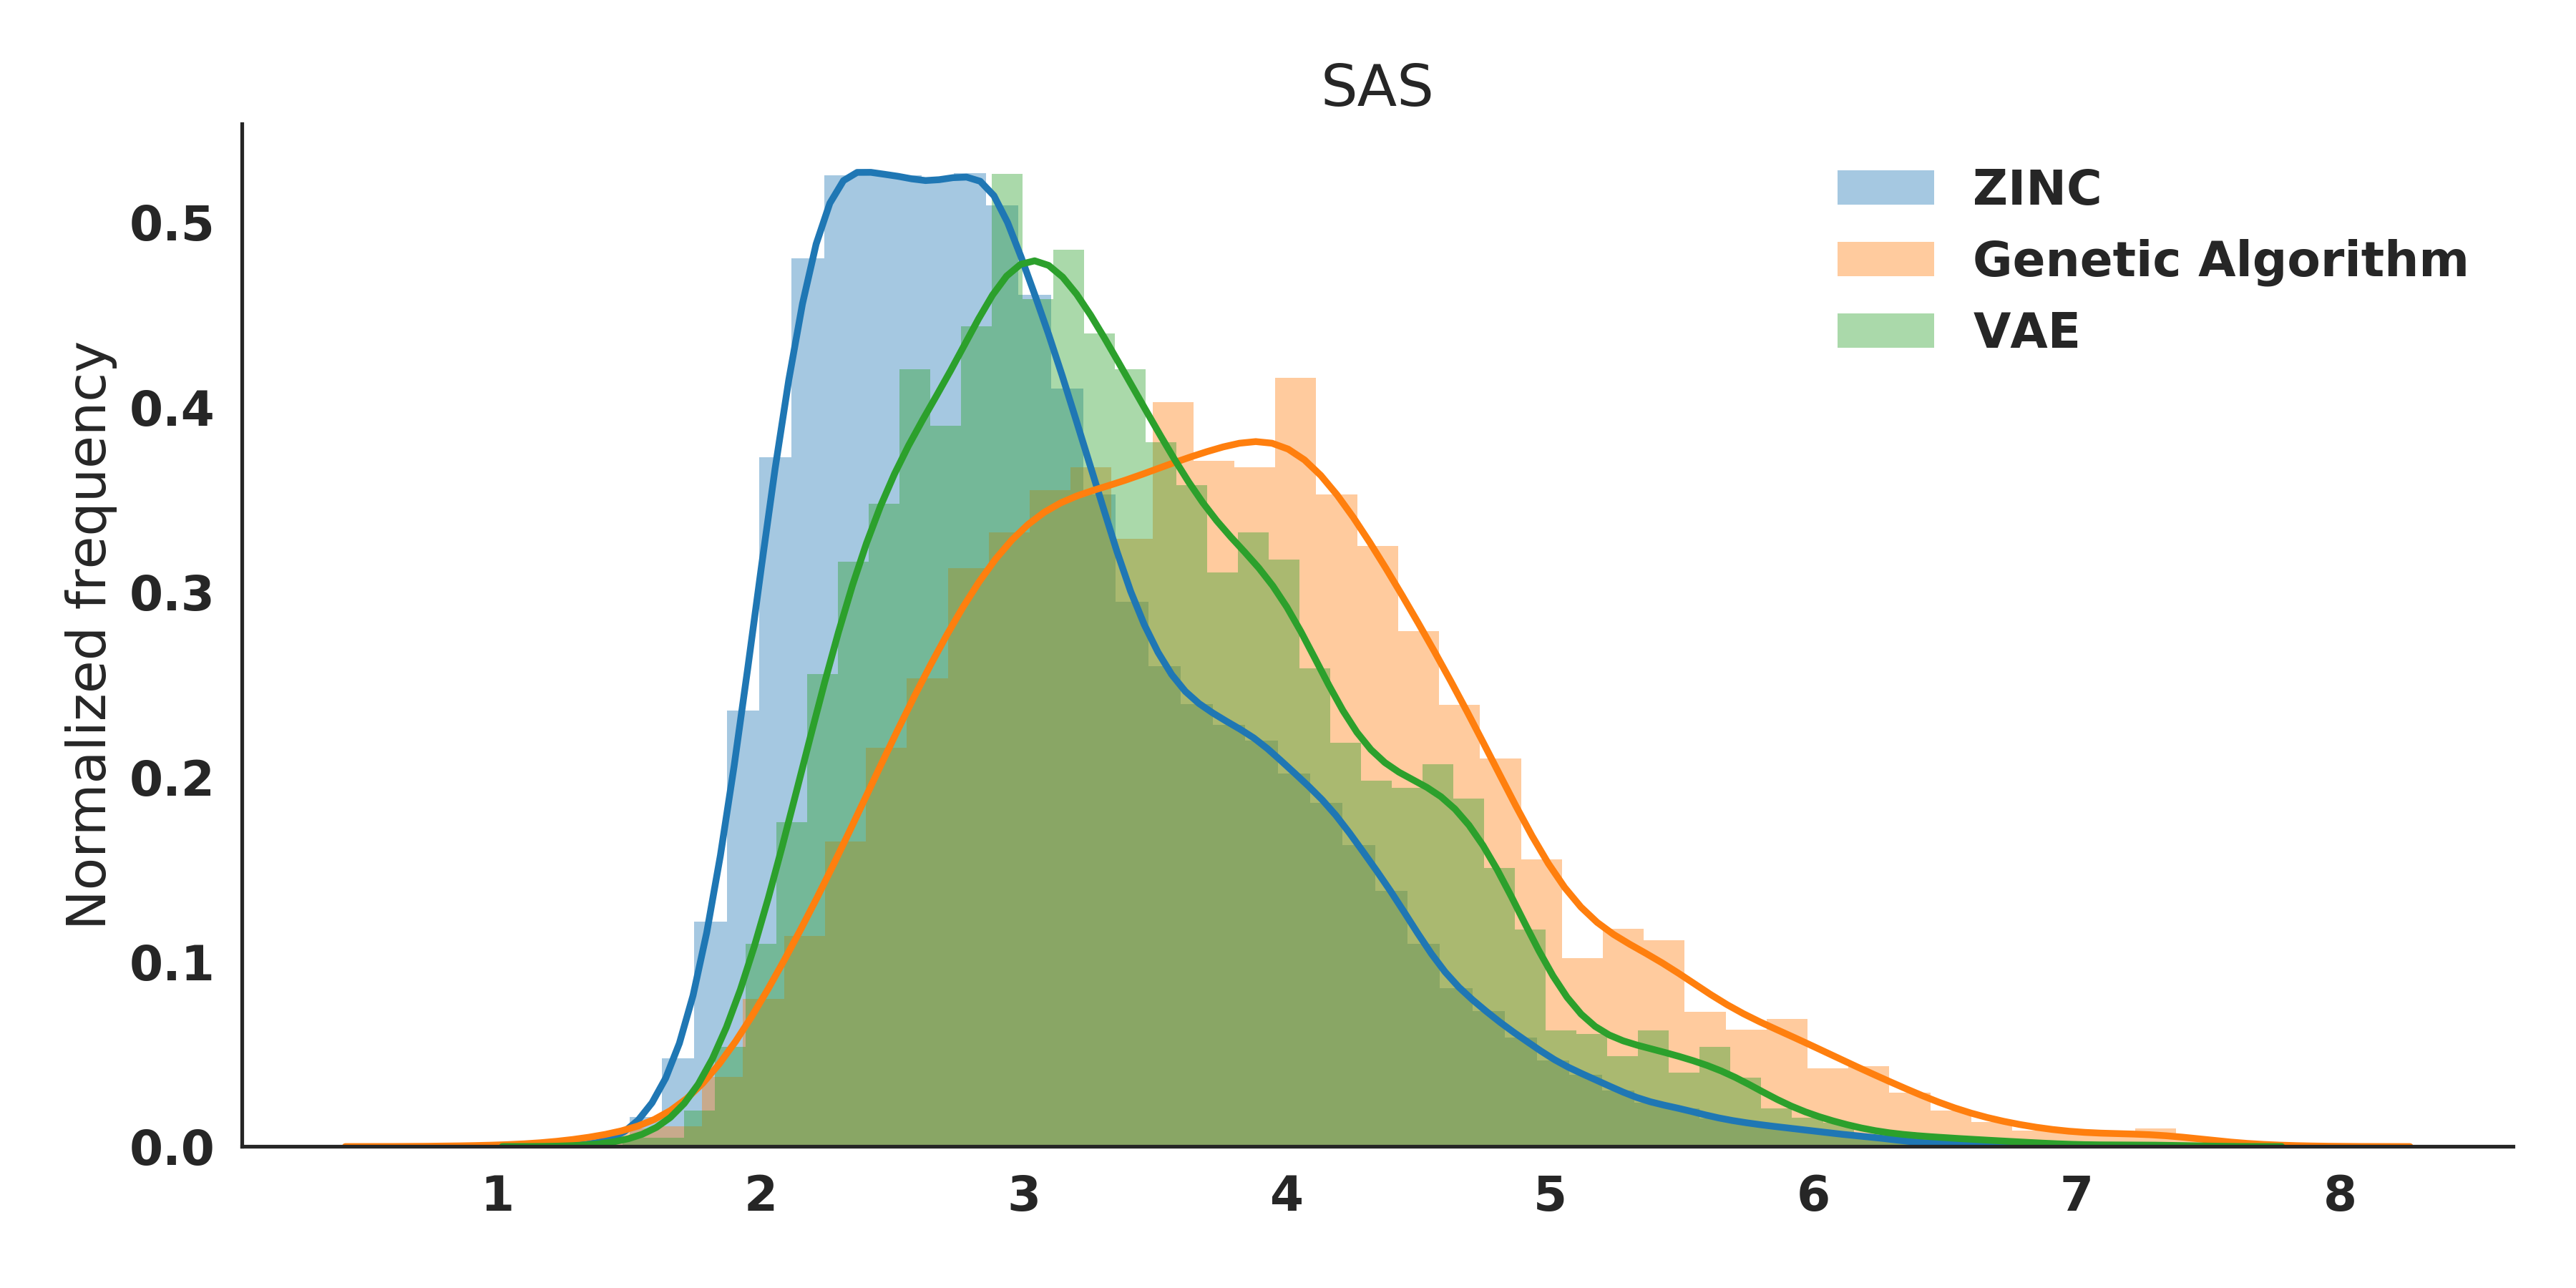
\includegraphics[width=0.3\columnwidth]{./SAS.png}
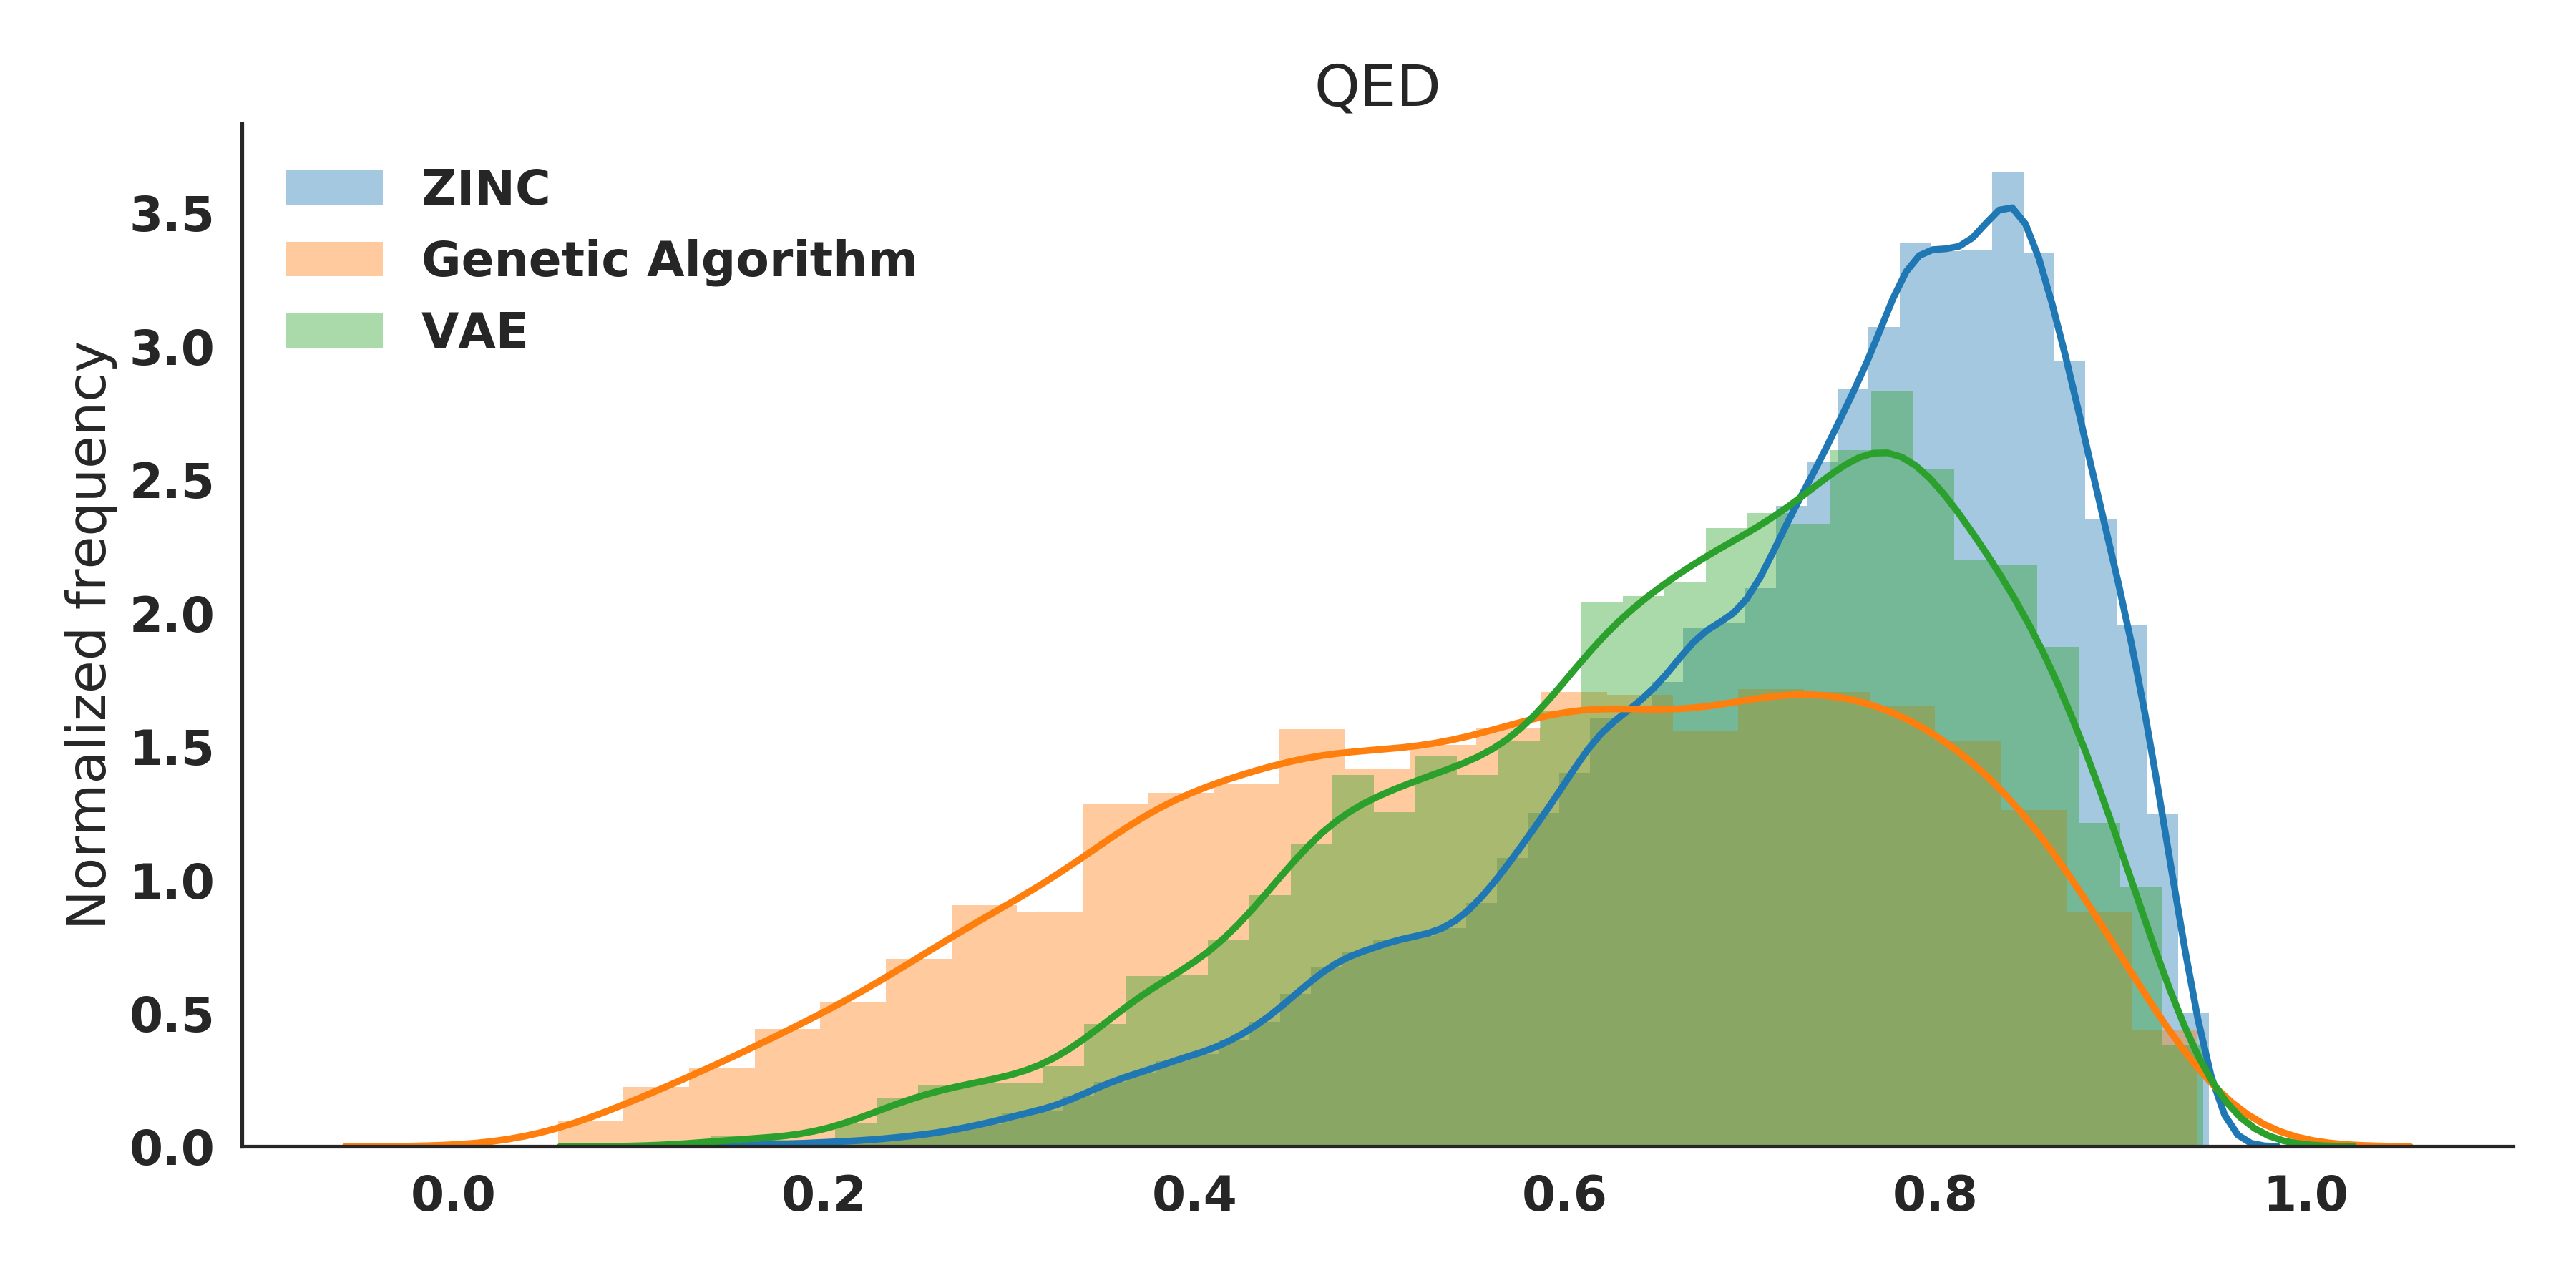
\includegraphics[width=0.3\columnwidth]{./QED.png}

\caption[KDE plots for distribution of logP, SAS, and QED properties]{
Histograms and KDE plots of the distribution of properties utilized in the jointly trained autoencoder (LogP, SAS, QED). Used to further showcase results from Table 2. For each property we compare the distribution of the source data (ZINC), a generatic algorithm and the VAE.}
\label{fig:prop_dists}
\end{figure}


\begin{figure}
\centering
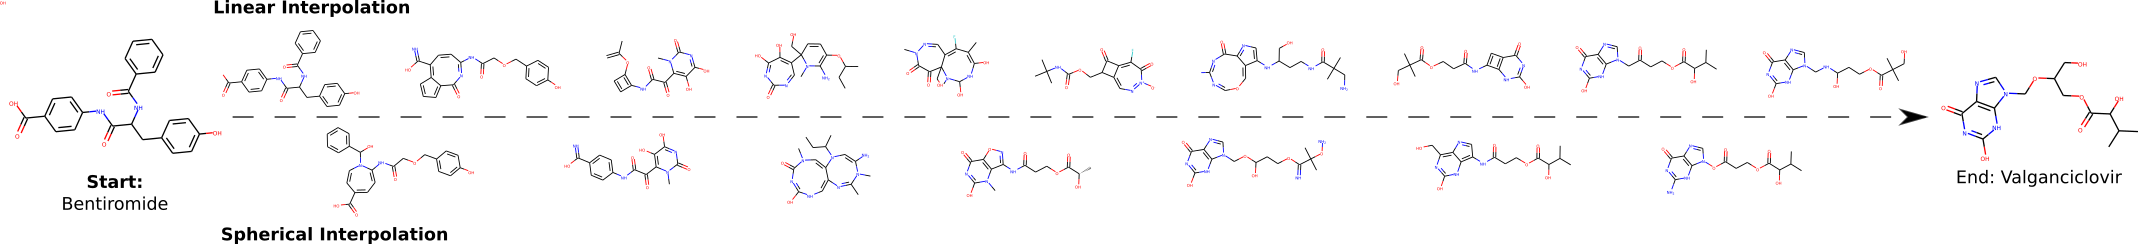
\includegraphics[width=\columnwidth]{./Slerp-lerp_compare.png}
\caption[Comparison of Interpolation Methods]{Comparison of between linear and spherical interpolation paths between two randomly selected FDA approved drugs. A constant step size was used.}
\label{fig:interpol_1}
\end{figure}


\begin{figure}[h]
\centering
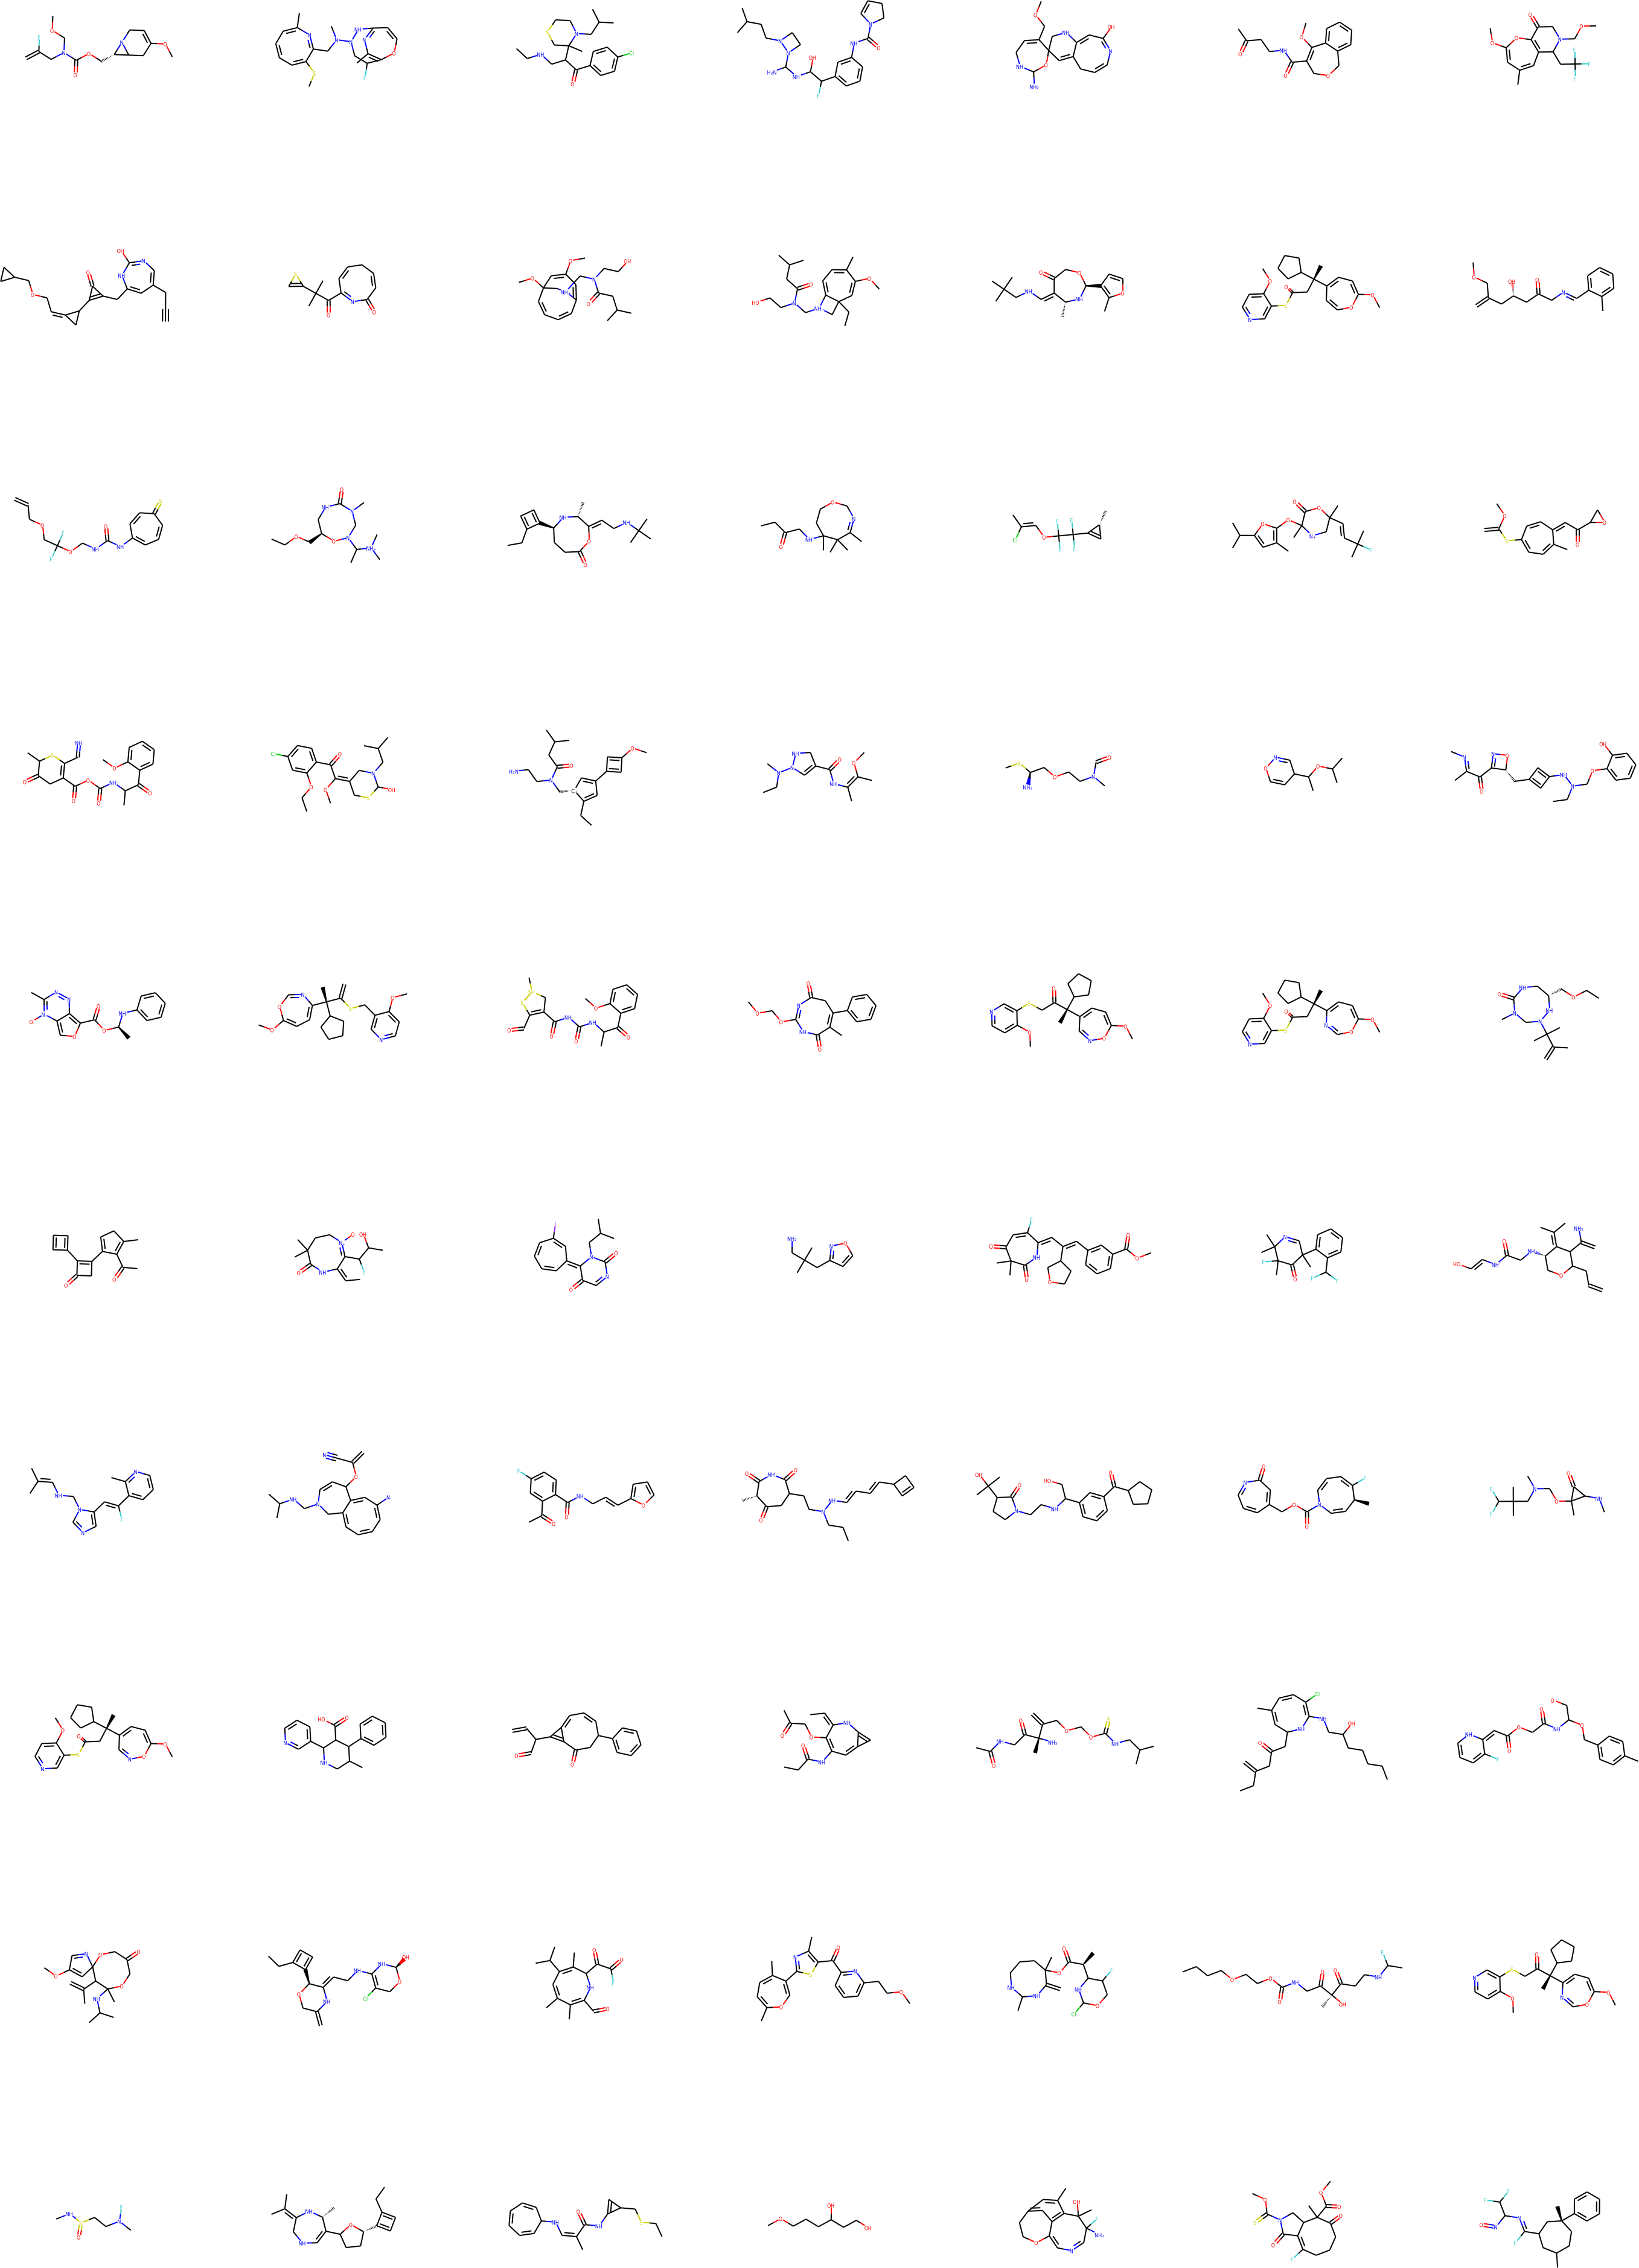
\includegraphics[width=0.9\columnwidth]{./VAE_random.png}
\caption[Random molecules sampled from Variational Autoencoder]{Molecules decoded from randomly-sampled points in the latent space of the ZINC VAE.}
\label{fig:random_3}
\end{figure}


\section{Supplementary Information for Chapter 5: Neural Networks for Predicting Reactions}

\begin{table}[ht]\label{tab:problem_training_similarity}
\centering
\caption{The Tanimoto similarity of the training set to problems Wade 8-47 and 8-48 used in the main article.}
\begin{tabular}{ccc}
\hline
 Problem number & Average Training Set & Highest Training Set \\
  & Tanimoto Similarity & Tanimoto Similarity \\
\hline
8-47a&0.30&0.94\\
8-47b&0.42&0.74\\
8-47c&0.47&0.86\\
8-47d&0.41&0.76\\
8-47e&0.47&0.88\\
8-47f&0.47&0.88\\
8-47g&0.35&0.65\\
8-47h&0.42&0.75\\
8-47i&0.43&0.80\\
8-47j&0.48&0.76\\
8-47l&0.44&0.77\\
8-47m&0.43&0.82\\
8-47n&0.45&0.75\\
8-47o&0.44&0.75\\
8-47p&0.44&0.76\\
\hline
8-48a&0.42&0.78\\
8-48b&0.42&0.77\\
8-48c&0.31&1.00\\
8-48d&0.34&0.54\\
8-48e&0.19&0.71\\
8-48f&0.20&0.66\\
8-48g&0.33&0.48\\
\hline
\end{tabular}
\end{table}


\section{Supplementary Information for Chapter 6: Neural Networks for Predicting Electron-Ionization Mass Spectrometry of Small Molecules}

\begin{figure}
  \centering
    \begin{subfigure}[b]{0.48\linewidth}
        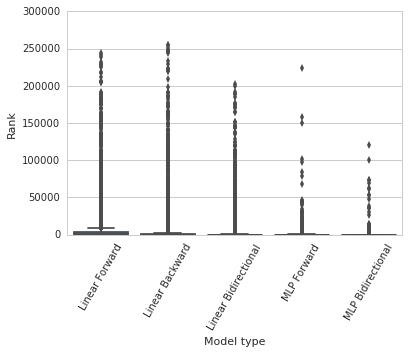
\includegraphics[width=\linewidth]{./model_all_results_boxplot_outliers.png}
        \caption{}
    \end{subfigure}
    \begin{subfigure}[b]{0.48\linewidth}
        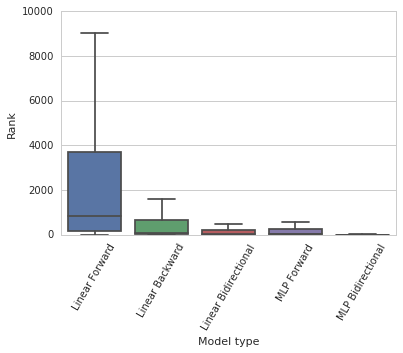
\includegraphics[width=\linewidth]{./model_all_results_boxplot.png}
        \caption{}
    \end{subfigure}
  \caption[Box Plot of Library Match Ranking Results]{
  The boxplot for all of the library matching ranks are shown in these figures.
  (a) shows the box plot distribution excluding outliers, while (b) shows the box plot distribution for all results including outliers.
  }
\end{figure}

\begin{figure}[h]
    \centering
    \begin{subfigure}[b]{0.48\linewidth}
        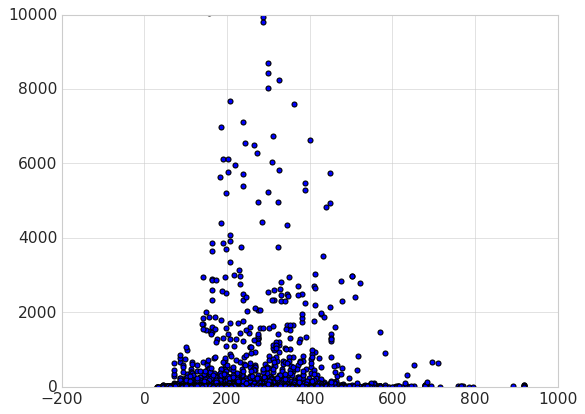
\includegraphics[width=\linewidth]{./mass_prediction_rank.png}
        \caption{}
    \end{subfigure}
    \begin{subfigure}[b]{0.48\linewidth}
        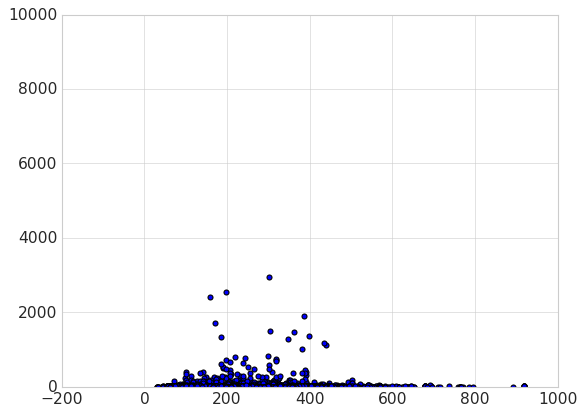
\includegraphics[width=\linewidth]{./mass_prediction_rank_mass_filter.png}
        \caption{}
    \end{subfigure}
    \caption[Ranks with and without mass filter]{
    Library matching ranks (y-axis) for all query spectra based on molecular mass (x-axis).
    (a) Shows the resulting ranks without the use of the mass filter, while (b) shows the resulting ranks with the mass filter.
    The matching rank improves significantly by using the mass filter, as indicated by the clustering of data towards the x-axis.
    This is especially the case for those spectra that are in the center of the mass range.}
    \label{fig:similarity_scatter_plots}
\end{figure}

\begin{figure}[h]
    \centering
    \begin{subfigure}[b]{0.48\linewidth}
        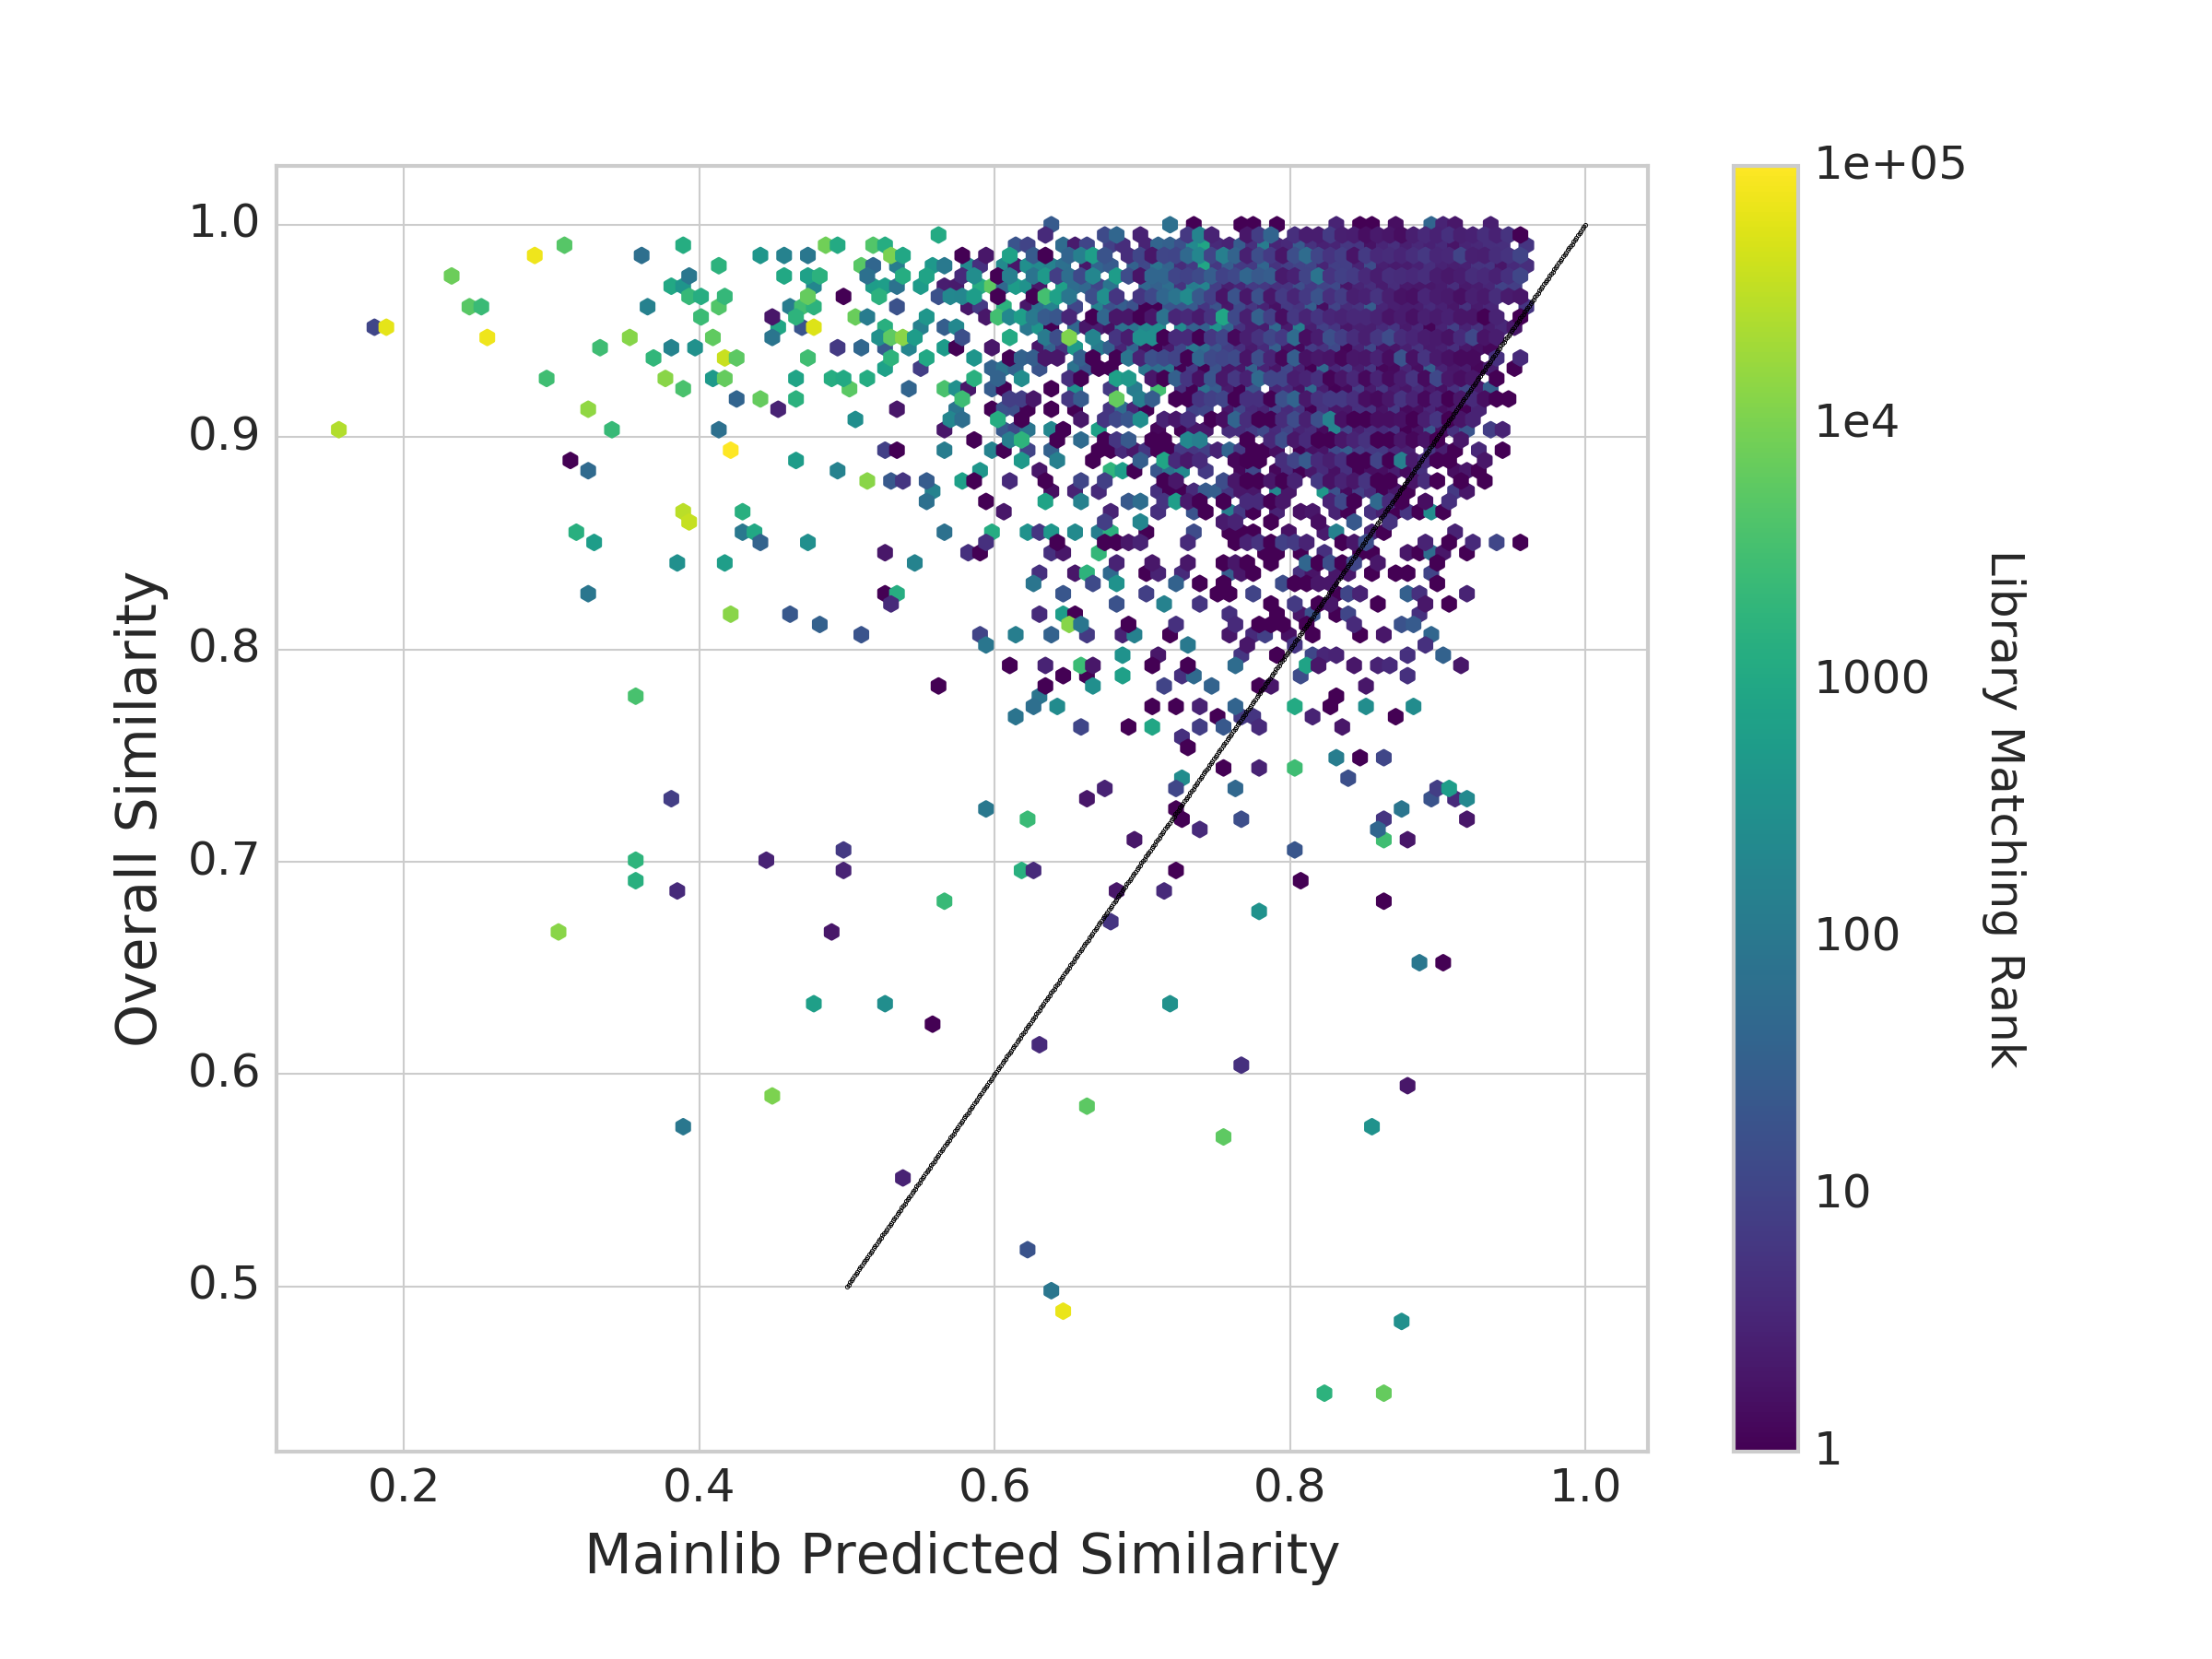
\includegraphics[width=\linewidth]{./mainlib_predicted_overall_similarity.png}
        \caption{}
    \end{subfigure}
    \begin{subfigure}[b]{0.48\linewidth}
        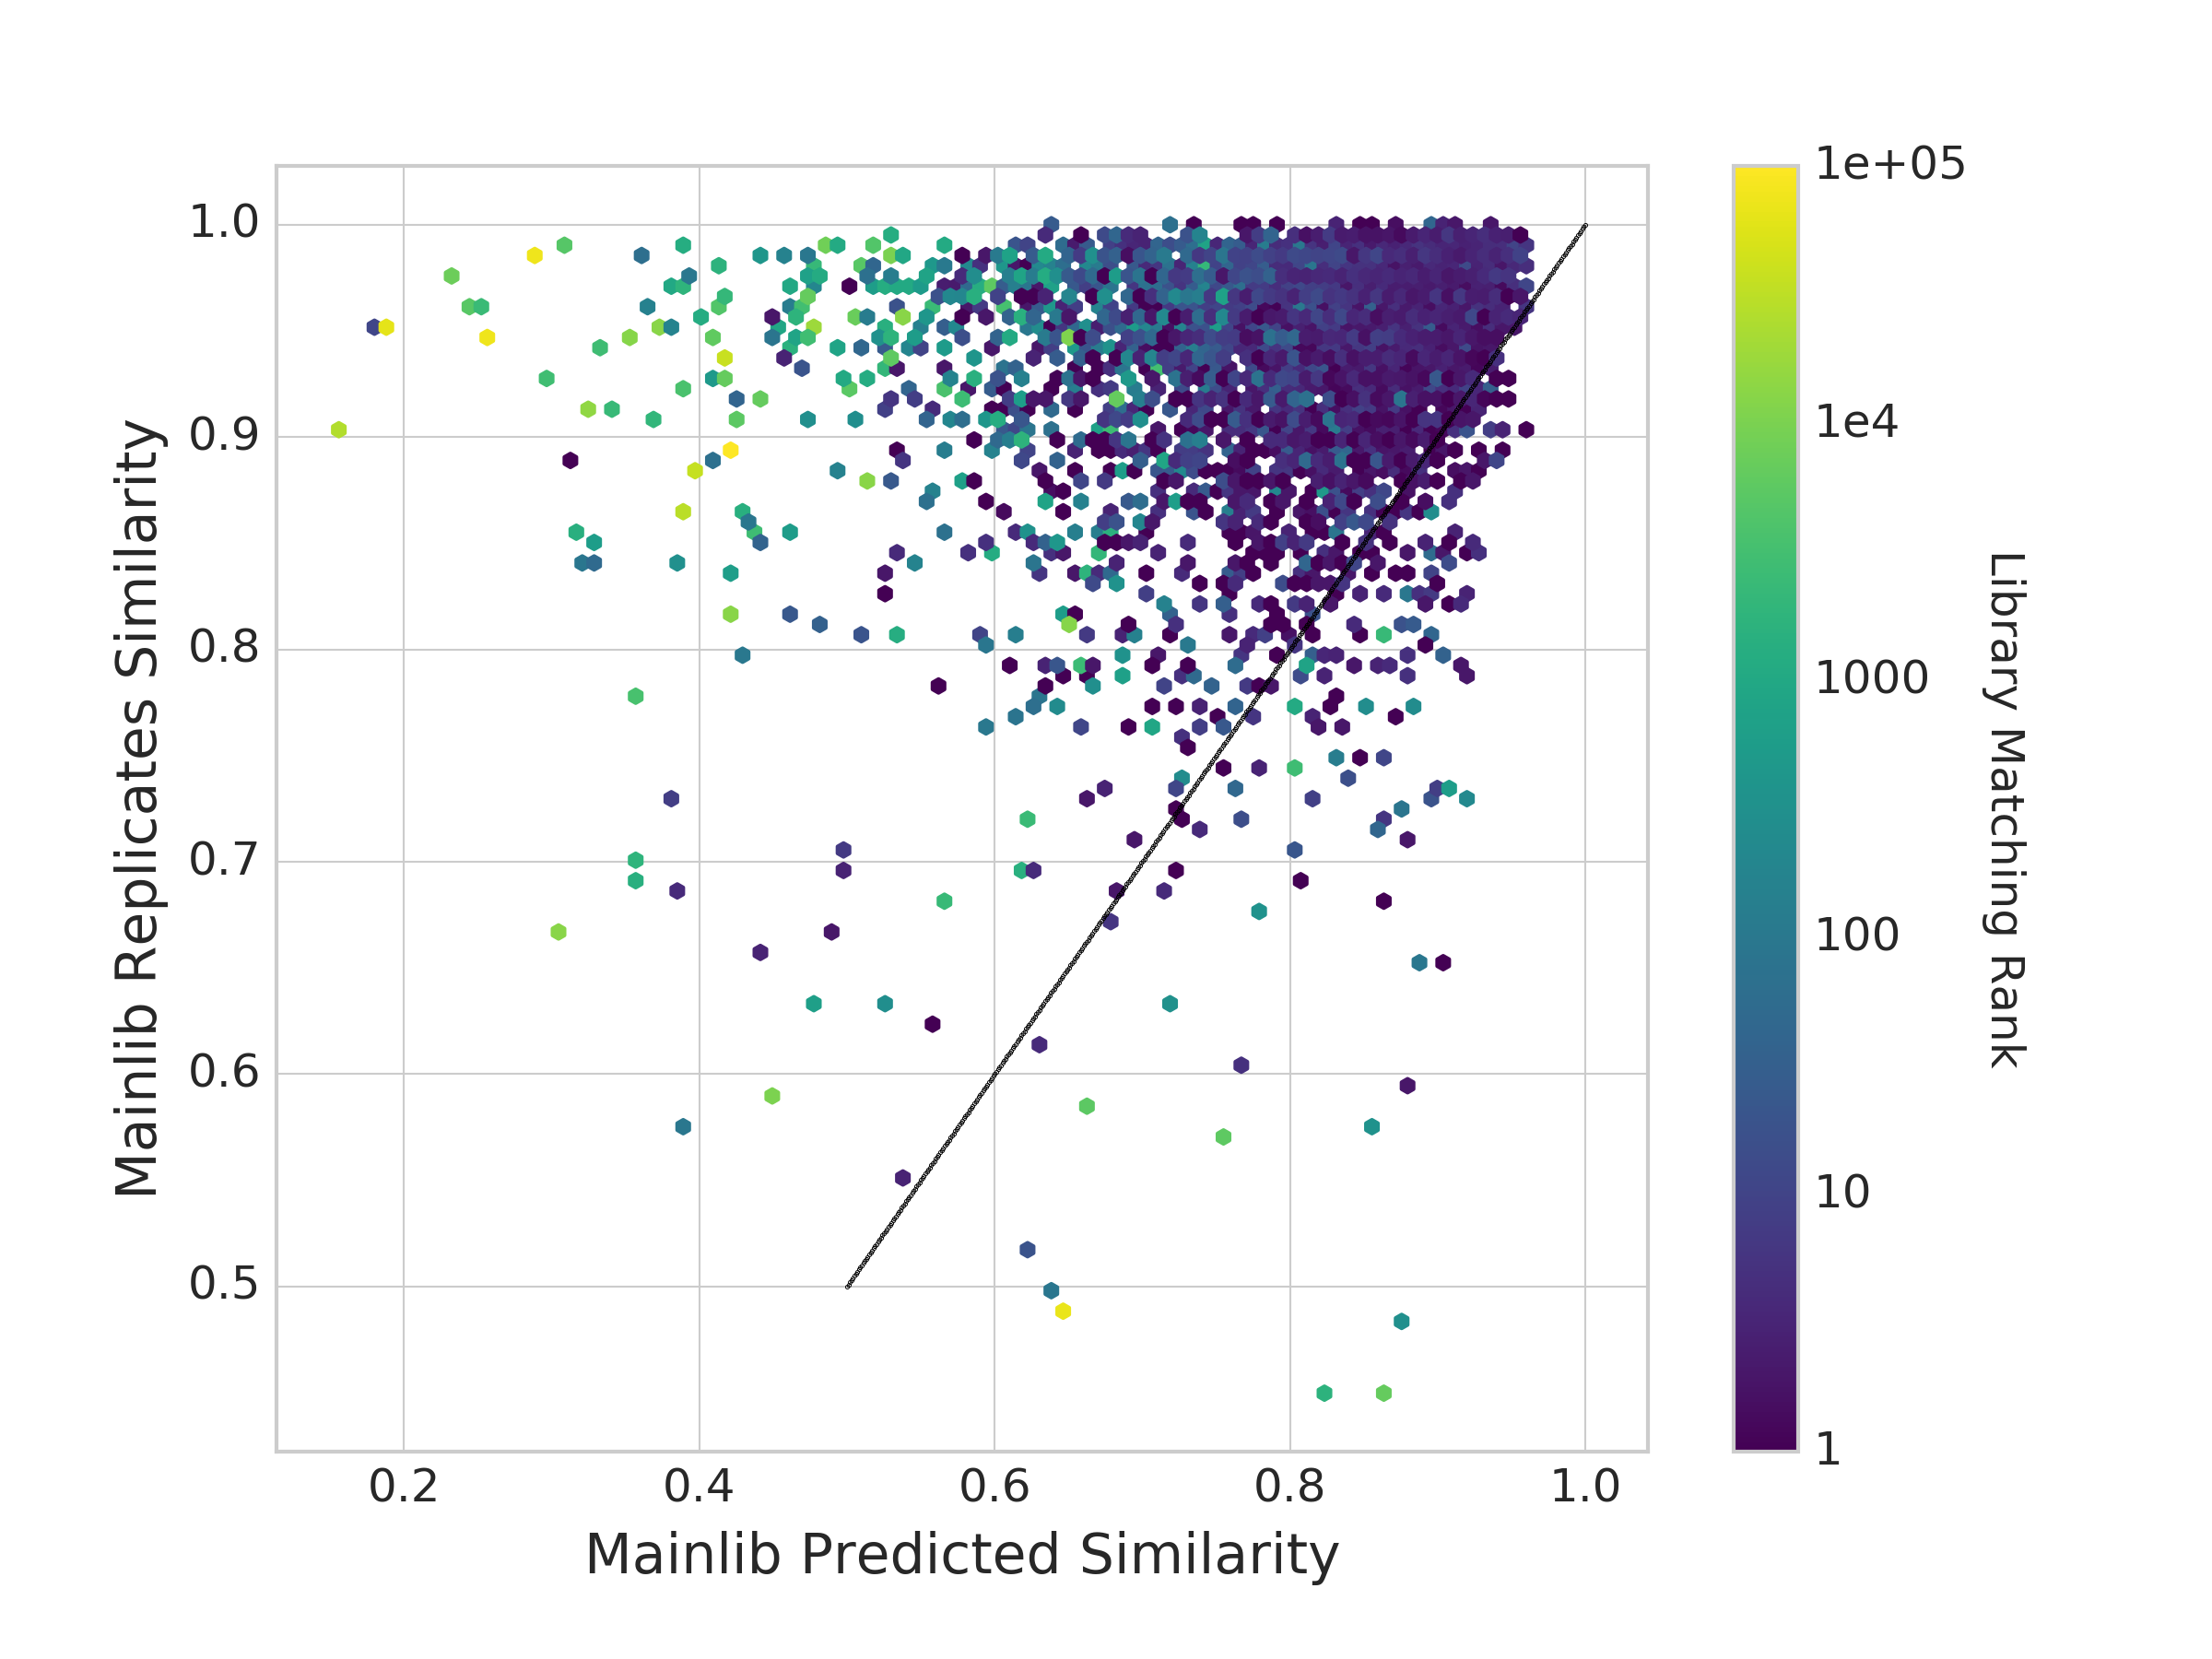
\includegraphics[width=\linewidth]{./main_predicted_main_replicates.png}
        \caption{}
    \end{subfigure}
    \\
    \begin{subfigure}[b]{0.48\linewidth}
        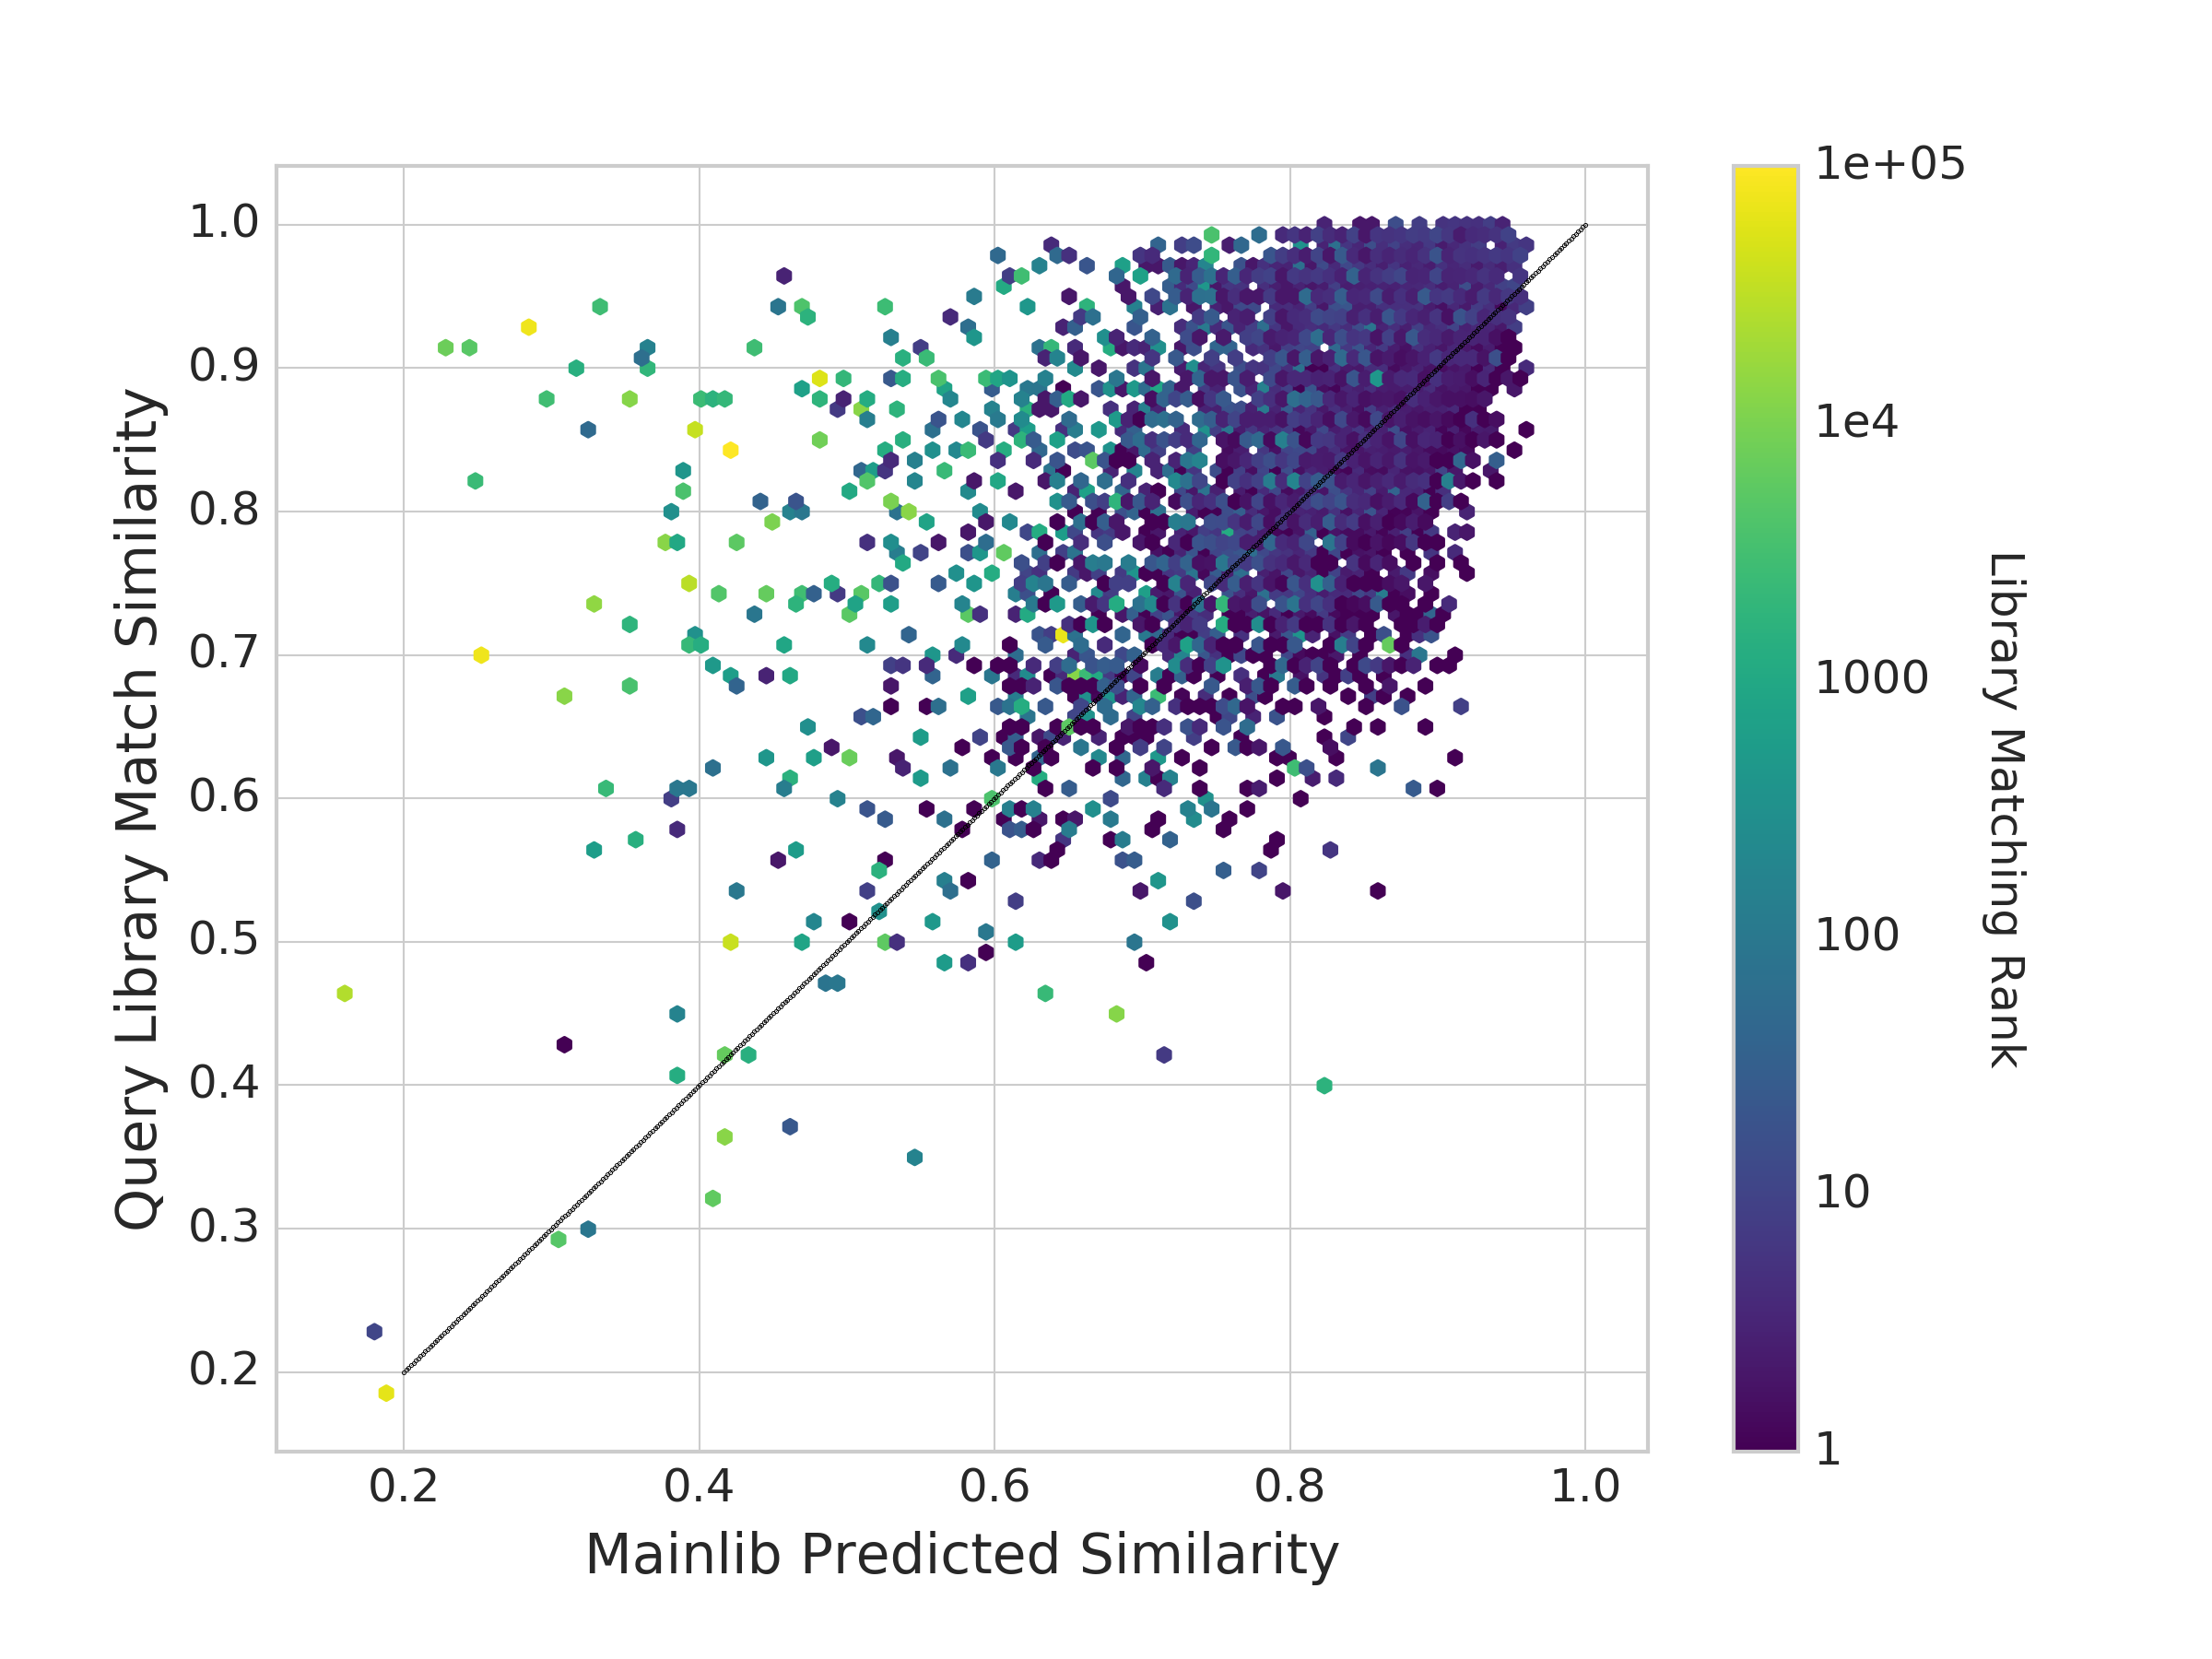
\includegraphics[width=\linewidth]{./main_predicted_query_libmatch.png}
        \caption{}
    \end{subfigure}
    \begin{subfigure}[b]{0.48\linewidth}
        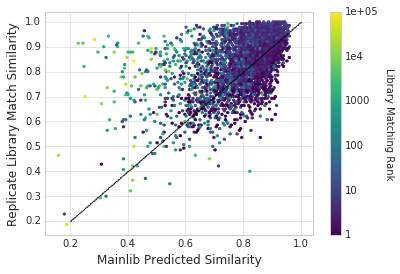
\includegraphics[width=\linewidth]{./main_predicted_replicates_libmatch.png}
        \caption{}
    \end{subfigure}
    \caption[Similarity Plots]{
    The above shows a collection of similarity plots for each molecule in the query set.
    The plots show a hex-bin heatmap, with Library matching rank representing the color of
    the hexbin for all plots.
    measuring the distances between spectra.
    (a) shows the distribution between Overall Similarity (i.e. the similarity between
     all recorded spectra for the same molecule) and predicted similarity.
     The ratio between these values is shown in Figure \ref{fig:similarity_analysis}.
    (b) compares the predicted similarity against the similarity of the main spectrum
    to the replicates spectra for the same molecule. This gives an indication of
    similar the predicted spectra is compared to the rest of the replicate spectra.
    (c) shows the distribution between the Predicted Similarity (x-axis) and the
    Query Library Match similarity. This gives an indication of how much more similar
    the query spectrum is to the library matched spectrum compared against
    the predicted similarity.
    (d) compares the similarity between the predicted similarity and the similarity
    between the replicates spectra to the library match spectra. The similarity between
    the replicates spectra and the library matched spectra gives an indication of the noise
    in the spectra for the molecule, and how that might have affect on the similarity matching.
    }
\end{figure}
